% Edit all prose, captions, and table values in this file.
% Figures: figures/ | References: iclr2027_conference.bib
% Numeric source audit: three-seed main-model aggregates supplied in Overleaf;
% seed-level provenance pending reconciliation. Do not infer extra figure runs.
\documentclass{article} % For LaTeX2e
\usepackage{iclr2027_conference,times}

% Optional math commands from https://github.com/goodfeli/dlbook_notation.
%%%%% NEW MATH DEFINITIONS %%%%%

\usepackage{amsmath,amsfonts,bm}

% Mark sections of captions for referring to divisions of figures
\newcommand{\figleft}{{\em (Left)}}
\newcommand{\figcenter}{{\em (Center)}}
\newcommand{\figright}{{\em (Right)}}
\newcommand{\figtop}{{\em (Top)}}
\newcommand{\figbottom}{{\em (Bottom)}}
\newcommand{\captiona}{{\em (a)}}
\newcommand{\captionb}{{\em (b)}}
\newcommand{\captionc}{{\em (c)}}
\newcommand{\captiond}{{\em (d)}}

% Highlight a newly defined term
\newcommand{\newterm}[1]{{\bf #1}}


% Figure reference, lower-case.
\def\figref#1{figure~\ref{#1}}
% Figure reference, capital. For start of sentence
\def\Figref#1{Figure~\ref{#1}}
\def\twofigref#1#2{figures \ref{#1} and \ref{#2}}
\def\quadfigref#1#2#3#4{figures \ref{#1}, \ref{#2}, \ref{#3} and \ref{#4}}
% Section reference, lower-case.
\def\secref#1{section~\ref{#1}}
% Section reference, capital.
\def\Secref#1{Section~\ref{#1}}
% Reference to two sections.
\def\twosecrefs#1#2{sections \ref{#1} and \ref{#2}}
% Reference to three sections.
\def\secrefs#1#2#3{sections \ref{#1}, \ref{#2} and \ref{#3}}
% Reference to an equation, lower-case.
\def\eqref#1{equation~\ref{#1}}
% Reference to an equation, upper case
\def\Eqref#1{Equation~\ref{#1}}
% A raw reference to an equation---avoid using if possible
\def\plaineqref#1{\ref{#1}}
% Reference to a chapter, lower-case.
\def\chapref#1{chapter~\ref{#1}}
% Reference to an equation, upper case.
\def\Chapref#1{Chapter~\ref{#1}}
% Reference to a range of chapters
\def\rangechapref#1#2{chapters\ref{#1}--\ref{#2}}
% Reference to an algorithm, lower-case.
\def\algref#1{algorithm~\ref{#1}}
% Reference to an algorithm, upper case.
\def\Algref#1{Algorithm~\ref{#1}}
\def\twoalgref#1#2{algorithms \ref{#1} and \ref{#2}}
\def\Twoalgref#1#2{Algorithms \ref{#1} and \ref{#2}}
% Reference to a part, lower case
\def\partref#1{part~\ref{#1}}
% Reference to a part, upper case
\def\Partref#1{Part~\ref{#1}}
\def\twopartref#1#2{parts \ref{#1} and \ref{#2}}

\def\ceil#1{\lceil #1 \rceil}
\def\floor#1{\lfloor #1 \rfloor}
\def\1{\bm{1}}
\newcommand{\train}{\mathcal{D}}
\newcommand{\valid}{\mathcal{D_{\mathrm{valid}}}}
\newcommand{\test}{\mathcal{D_{\mathrm{test}}}}

\def\eps{{\epsilon}}


% Random variables
\def\reta{{\textnormal{$\eta$}}}
\def\ra{{\textnormal{a}}}
\def\rb{{\textnormal{b}}}
\def\rc{{\textnormal{c}}}
\def\rd{{\textnormal{d}}}
\def\re{{\textnormal{e}}}
\def\rf{{\textnormal{f}}}
\def\rg{{\textnormal{g}}}
\def\rh{{\textnormal{h}}}
\def\ri{{\textnormal{i}}}
\def\rj{{\textnormal{j}}}
\def\rk{{\textnormal{k}}}
\def\rl{{\textnormal{l}}}
% rm is already a command, just don't name any random variables m
\def\rn{{\textnormal{n}}}
\def\ro{{\textnormal{o}}}
\def\rp{{\textnormal{p}}}
\def\rq{{\textnormal{q}}}
\def\rr{{\textnormal{r}}}
\def\rs{{\textnormal{s}}}
\def\rt{{\textnormal{t}}}
\def\ru{{\textnormal{u}}}
\def\rv{{\textnormal{v}}}
\def\rw{{\textnormal{w}}}
\def\rx{{\textnormal{x}}}
\def\ry{{\textnormal{y}}}
\def\rz{{\textnormal{z}}}

% Random vectors
\def\rvepsilon{{\mathbf{\epsilon}}}
\def\rvtheta{{\mathbf{\theta}}}
\def\rva{{\mathbf{a}}}
\def\rvb{{\mathbf{b}}}
\def\rvc{{\mathbf{c}}}
\def\rvd{{\mathbf{d}}}
\def\rve{{\mathbf{e}}}
\def\rvf{{\mathbf{f}}}
\def\rvg{{\mathbf{g}}}
\def\rvh{{\mathbf{h}}}
\def\rvu{{\mathbf{i}}}
\def\rvj{{\mathbf{j}}}
\def\rvk{{\mathbf{k}}}
\def\rvl{{\mathbf{l}}}
\def\rvm{{\mathbf{m}}}
\def\rvn{{\mathbf{n}}}
\def\rvo{{\mathbf{o}}}
\def\rvp{{\mathbf{p}}}
\def\rvq{{\mathbf{q}}}
\def\rvr{{\mathbf{r}}}
\def\rvs{{\mathbf{s}}}
\def\rvt{{\mathbf{t}}}
\def\rvu{{\mathbf{u}}}
\def\rvv{{\mathbf{v}}}
\def\rvw{{\mathbf{w}}}
\def\rvx{{\mathbf{x}}}
\def\rvy{{\mathbf{y}}}
\def\rvz{{\mathbf{z}}}

% Elements of random vectors
\def\erva{{\textnormal{a}}}
\def\ervb{{\textnormal{b}}}
\def\ervc{{\textnormal{c}}}
\def\ervd{{\textnormal{d}}}
\def\erve{{\textnormal{e}}}
\def\ervf{{\textnormal{f}}}
\def\ervg{{\textnormal{g}}}
\def\ervh{{\textnormal{h}}}
\def\ervi{{\textnormal{i}}}
\def\ervj{{\textnormal{j}}}
\def\ervk{{\textnormal{k}}}
\def\ervl{{\textnormal{l}}}
\def\ervm{{\textnormal{m}}}
\def\ervn{{\textnormal{n}}}
\def\ervo{{\textnormal{o}}}
\def\ervp{{\textnormal{p}}}
\def\ervq{{\textnormal{q}}}
\def\ervr{{\textnormal{r}}}
\def\ervs{{\textnormal{s}}}
\def\ervt{{\textnormal{t}}}
\def\ervu{{\textnormal{u}}}
\def\ervv{{\textnormal{v}}}
\def\ervw{{\textnormal{w}}}
\def\ervx{{\textnormal{x}}}
\def\ervy{{\textnormal{y}}}
\def\ervz{{\textnormal{z}}}

% Random matrices
\def\rmA{{\mathbf{A}}}
\def\rmB{{\mathbf{B}}}
\def\rmC{{\mathbf{C}}}
\def\rmD{{\mathbf{D}}}
\def\rmE{{\mathbf{E}}}
\def\rmF{{\mathbf{F}}}
\def\rmG{{\mathbf{G}}}
\def\rmH{{\mathbf{H}}}
\def\rmI{{\mathbf{I}}}
\def\rmJ{{\mathbf{J}}}
\def\rmK{{\mathbf{K}}}
\def\rmL{{\mathbf{L}}}
\def\rmM{{\mathbf{M}}}
\def\rmN{{\mathbf{N}}}
\def\rmO{{\mathbf{O}}}
\def\rmP{{\mathbf{P}}}
\def\rmQ{{\mathbf{Q}}}
\def\rmR{{\mathbf{R}}}
\def\rmS{{\mathbf{S}}}
\def\rmT{{\mathbf{T}}}
\def\rmU{{\mathbf{U}}}
\def\rmV{{\mathbf{V}}}
\def\rmW{{\mathbf{W}}}
\def\rmX{{\mathbf{X}}}
\def\rmY{{\mathbf{Y}}}
\def\rmZ{{\mathbf{Z}}}

% Elements of random matrices
\def\ermA{{\textnormal{A}}}
\def\ermB{{\textnormal{B}}}
\def\ermC{{\textnormal{C}}}
\def\ermD{{\textnormal{D}}}
\def\ermE{{\textnormal{E}}}
\def\ermF{{\textnormal{F}}}
\def\ermG{{\textnormal{G}}}
\def\ermH{{\textnormal{H}}}
\def\ermI{{\textnormal{I}}}
\def\ermJ{{\textnormal{J}}}
\def\ermK{{\textnormal{K}}}
\def\ermL{{\textnormal{L}}}
\def\ermM{{\textnormal{M}}}
\def\ermN{{\textnormal{N}}}
\def\ermO{{\textnormal{O}}}
\def\ermP{{\textnormal{P}}}
\def\ermQ{{\textnormal{Q}}}
\def\ermR{{\textnormal{R}}}
\def\ermS{{\textnormal{S}}}
\def\ermT{{\textnormal{T}}}
\def\ermU{{\textnormal{U}}}
\def\ermV{{\textnormal{V}}}
\def\ermW{{\textnormal{W}}}
\def\ermX{{\textnormal{X}}}
\def\ermY{{\textnormal{Y}}}
\def\ermZ{{\textnormal{Z}}}

% Vectors
\def\vzero{{\bm{0}}}
\def\vone{{\bm{1}}}
\def\vmu{{\bm{\mu}}}
\def\vtheta{{\bm{\theta}}}
\def\va{{\bm{a}}}
\def\vb{{\bm{b}}}
\def\vc{{\bm{c}}}
\def\vd{{\bm{d}}}
\def\ve{{\bm{e}}}
\def\vf{{\bm{f}}}
\def\vg{{\bm{g}}}
\def\vh{{\bm{h}}}
\def\vi{{\bm{i}}}
\def\vj{{\bm{j}}}
\def\vk{{\bm{k}}}
\def\vl{{\bm{l}}}
\def\vm{{\bm{m}}}
\def\vn{{\bm{n}}}
\def\vo{{\bm{o}}}
\def\vp{{\bm{p}}}
\def\vq{{\bm{q}}}
\def\vr{{\bm{r}}}
\def\vs{{\bm{s}}}
\def\vt{{\bm{t}}}
\def\vu{{\bm{u}}}
\def\vv{{\bm{v}}}
\def\vw{{\bm{w}}}
\def\vx{{\bm{x}}}
\def\vy{{\bm{y}}}
\def\vz{{\bm{z}}}

% Elements of vectors
\def\evalpha{{\alpha}}
\def\evbeta{{\beta}}
\def\evepsilon{{\epsilon}}
\def\evlambda{{\lambda}}
\def\evomega{{\omega}}
\def\evmu{{\mu}}
\def\evpsi{{\psi}}
\def\evsigma{{\sigma}}
\def\evtheta{{\theta}}
\def\eva{{a}}
\def\evb{{b}}
\def\evc{{c}}
\def\evd{{d}}
\def\eve{{e}}
\def\evf{{f}}
\def\evg{{g}}
\def\evh{{h}}
\def\evi{{i}}
\def\evj{{j}}
\def\evk{{k}}
\def\evl{{l}}
\def\evm{{m}}
\def\evn{{n}}
\def\evo{{o}}
\def\evp{{p}}
\def\evq{{q}}
\def\evr{{r}}
\def\evs{{s}}
\def\evt{{t}}
\def\evu{{u}}
\def\evv{{v}}
\def\evw{{w}}
\def\evx{{x}}
\def\evy{{y}}
\def\evz{{z}}

% Matrix
\def\mA{{\bm{A}}}
\def\mB{{\bm{B}}}
\def\mC{{\bm{C}}}
\def\mD{{\bm{D}}}
\def\mE{{\bm{E}}}
\def\mF{{\bm{F}}}
\def\mG{{\bm{G}}}
\def\mH{{\bm{H}}}
\def\mI{{\bm{I}}}
\def\mJ{{\bm{J}}}
\def\mK{{\bm{K}}}
\def\mL{{\bm{L}}}
\def\mM{{\bm{M}}}
\def\mN{{\bm{N}}}
\def\mO{{\bm{O}}}
\def\mP{{\bm{P}}}
\def\mQ{{\bm{Q}}}
\def\mR{{\bm{R}}}
\def\mS{{\bm{S}}}
\def\mT{{\bm{T}}}
\def\mU{{\bm{U}}}
\def\mV{{\bm{V}}}
\def\mW{{\bm{W}}}
\def\mX{{\bm{X}}}
\def\mY{{\bm{Y}}}
\def\mZ{{\bm{Z}}}
\def\mBeta{{\bm{\beta}}}
\def\mPhi{{\bm{\Phi}}}
\def\mLambda{{\bm{\Lambda}}}
\def\mSigma{{\bm{\Sigma}}}

% Tensor
\DeclareMathAlphabet{\mathsfit}{\encodingdefault}{\sfdefault}{m}{sl}
\SetMathAlphabet{\mathsfit}{bold}{\encodingdefault}{\sfdefault}{bx}{n}
\newcommand{\tens}[1]{\bm{\mathsfit{#1}}}
\def\tA{{\tens{A}}}
\def\tB{{\tens{B}}}
\def\tC{{\tens{C}}}
\def\tD{{\tens{D}}}
\def\tE{{\tens{E}}}
\def\tF{{\tens{F}}}
\def\tG{{\tens{G}}}
\def\tH{{\tens{H}}}
\def\tI{{\tens{I}}}
\def\tJ{{\tens{J}}}
\def\tK{{\tens{K}}}
\def\tL{{\tens{L}}}
\def\tM{{\tens{M}}}
\def\tN{{\tens{N}}}
\def\tO{{\tens{O}}}
\def\tP{{\tens{P}}}
\def\tQ{{\tens{Q}}}
\def\tR{{\tens{R}}}
\def\tS{{\tens{S}}}
\def\tT{{\tens{T}}}
\def\tU{{\tens{U}}}
\def\tV{{\tens{V}}}
\def\tW{{\tens{W}}}
\def\tX{{\tens{X}}}
\def\tY{{\tens{Y}}}
\def\tZ{{\tens{Z}}}


% Graph
\def\gA{{\mathcal{A}}}
\def\gB{{\mathcal{B}}}
\def\gC{{\mathcal{C}}}
\def\gD{{\mathcal{D}}}
\def\gE{{\mathcal{E}}}
\def\gF{{\mathcal{F}}}
\def\gG{{\mathcal{G}}}
\def\gH{{\mathcal{H}}}
\def\gI{{\mathcal{I}}}
\def\gJ{{\mathcal{J}}}
\def\gK{{\mathcal{K}}}
\def\gL{{\mathcal{L}}}
\def\gM{{\mathcal{M}}}
\def\gN{{\mathcal{N}}}
\def\gO{{\mathcal{O}}}
\def\gP{{\mathcal{P}}}
\def\gQ{{\mathcal{Q}}}
\def\gR{{\mathcal{R}}}
\def\gS{{\mathcal{S}}}
\def\gT{{\mathcal{T}}}
\def\gU{{\mathcal{U}}}
\def\gV{{\mathcal{V}}}
\def\gW{{\mathcal{W}}}
\def\gX{{\mathcal{X}}}
\def\gY{{\mathcal{Y}}}
\def\gZ{{\mathcal{Z}}}

% Sets
\def\sA{{\mathbb{A}}}
\def\sB{{\mathbb{B}}}
\def\sC{{\mathbb{C}}}
\def\sD{{\mathbb{D}}}
% Don't use a set called E, because this would be the same as our symbol
% for expectation.
\def\sF{{\mathbb{F}}}
\def\sG{{\mathbb{G}}}
\def\sH{{\mathbb{H}}}
\def\sI{{\mathbb{I}}}
\def\sJ{{\mathbb{J}}}
\def\sK{{\mathbb{K}}}
\def\sL{{\mathbb{L}}}
\def\sM{{\mathbb{M}}}
\def\sN{{\mathbb{N}}}
\def\sO{{\mathbb{O}}}
\def\sP{{\mathbb{P}}}
\def\sQ{{\mathbb{Q}}}
\def\sR{{\mathbb{R}}}
\def\sS{{\mathbb{S}}}
\def\sT{{\mathbb{T}}}
\def\sU{{\mathbb{U}}}
\def\sV{{\mathbb{V}}}
\def\sW{{\mathbb{W}}}
\def\sX{{\mathbb{X}}}
\def\sY{{\mathbb{Y}}}
\def\sZ{{\mathbb{Z}}}

% Entries of a matrix
\def\emLambda{{\Lambda}}
\def\emA{{A}}
\def\emB{{B}}
\def\emC{{C}}
\def\emD{{D}}
\def\emE{{E}}
\def\emF{{F}}
\def\emG{{G}}
\def\emH{{H}}
\def\emI{{I}}
\def\emJ{{J}}
\def\emK{{K}}
\def\emL{{L}}
\def\emM{{M}}
\def\emN{{N}}
\def\emO{{O}}
\def\emP{{P}}
\def\emQ{{Q}}
\def\emR{{R}}
\def\emS{{S}}
\def\emT{{T}}
\def\emU{{U}}
\def\emV{{V}}
\def\emW{{W}}
\def\emX{{X}}
\def\emY{{Y}}
\def\emZ{{Z}}
\def\emSigma{{\Sigma}}

% entries of a tensor
% Same font as tensor, without \bm wrapper
\newcommand{\etens}[1]{\mathsfit{#1}}
\def\etLambda{{\etens{\Lambda}}}
\def\etA{{\etens{A}}}
\def\etB{{\etens{B}}}
\def\etC{{\etens{C}}}
\def\etD{{\etens{D}}}
\def\etE{{\etens{E}}}
\def\etF{{\etens{F}}}
\def\etG{{\etens{G}}}
\def\etH{{\etens{H}}}
\def\etI{{\etens{I}}}
\def\etJ{{\etens{J}}}
\def\etK{{\etens{K}}}
\def\etL{{\etens{L}}}
\def\etM{{\etens{M}}}
\def\etN{{\etens{N}}}
\def\etO{{\etens{O}}}
\def\etP{{\etens{P}}}
\def\etQ{{\etens{Q}}}
\def\etR{{\etens{R}}}
\def\etS{{\etens{S}}}
\def\etT{{\etens{T}}}
\def\etU{{\etens{U}}}
\def\etV{{\etens{V}}}
\def\etW{{\etens{W}}}
\def\etX{{\etens{X}}}
\def\etY{{\etens{Y}}}
\def\etZ{{\etens{Z}}}

% The true underlying data generating distribution
\newcommand{\pdata}{p_{\rm{data}}}
% The empirical distribution defined by the training set
\newcommand{\ptrain}{\hat{p}_{\rm{data}}}
\newcommand{\Ptrain}{\hat{P}_{\rm{data}}}
% The model distribution
\newcommand{\pmodel}{p_{\rm{model}}}
\newcommand{\Pmodel}{P_{\rm{model}}}
\newcommand{\ptildemodel}{\tilde{p}_{\rm{model}}}
% Stochastic autoencoder distributions
\newcommand{\pencode}{p_{\rm{encoder}}}
\newcommand{\pdecode}{p_{\rm{decoder}}}
\newcommand{\precons}{p_{\rm{reconstruct}}}

\newcommand{\laplace}{\mathrm{Laplace}} % Laplace distribution

\newcommand{\E}{\mathbb{E}}
\newcommand{\Ls}{\mathcal{L}}
\newcommand{\R}{\mathbb{R}}
\newcommand{\emp}{\tilde{p}}
\newcommand{\lr}{\alpha}
\newcommand{\reg}{\lambda}
\newcommand{\rect}{\mathrm{rectifier}}
\newcommand{\softmax}{\mathrm{softmax}}
\newcommand{\sigmoid}{\sigma}
\newcommand{\softplus}{\zeta}
\newcommand{\KL}{D_{\mathrm{KL}}}
\newcommand{\Var}{\mathrm{Var}}
\newcommand{\standarderror}{\mathrm{SE}}
\newcommand{\Cov}{\mathrm{Cov}}
% Wolfram Mathworld says $L^2$ is for function spaces and $\ell^2$ is for vectors
% But then they seem to use $L^2$ for vectors throughout the site, and so does
% wikipedia.
\newcommand{\normlzero}{L^0}
\newcommand{\normlone}{L^1}
\newcommand{\normltwo}{L^2}
\newcommand{\normlp}{L^p}
\newcommand{\normmax}{L^\infty}

\newcommand{\parents}{Pa} % See usage in notation.tex. Chosen to match Daphne's book.

\DeclareMathOperator*{\argmax}{arg\,max}
\DeclareMathOperator*{\argmin}{arg\,min}

\DeclareMathOperator{\sign}{sign}
\DeclareMathOperator{\Tr}{Tr}
\let\ab\allowbreak



\usepackage{hyperref}

\definecolor{citeblue}{HTML}{456BCF}

\hypersetup{
  colorlinks=true,
  breaklinks=true,
  linkcolor=citeblue,
  citecolor=citeblue,
  urlcolor=citeblue
}


\usepackage{xcolor}
\definecolor{cvprblue}{rgb}{0.21,0.49,0.74}
\definecolor{jonigold}{rgb}{0.85,0.65,0.00}

% Review markup is hidden in the compiled manuscript.
\newcommand{\newcomment}[1]{}
\newcommand{\reviewnote}[2]{}
\newcommand{\newcommentRTwo}[1]{}
\newcommand{\newcommentRTwoShow}[1]{}

% Optional: uncomment the matching block below to show a round's comments again.
%\renewcommand{\newcomment}[1]{%
%  \textcolor{cvprblue}{\textbf{[Sean:} #1\textbf{]}}%
%}
%\renewcommand{\reviewnote}[2]{%
%  \textcolor{jonigold}{\textbf{[#1:} #2\textbf{]}}%
%}
%\renewcommand{\newcommentRTwo}[1]{%
%  \textcolor{cvprblue}{\textbf{[Sean:} #1\textbf{]}}%
%}


\usepackage{hyperref}
%\hypersetup{hidelinks}
\usepackage{url}
\usepackage{booktabs}
\usepackage{graphicx}
\usepackage{capt-of} % captionof without overriding the conference caption style
\usepackage{flafter} % A figure must not precede its source position.
\usepackage{placeins}
\usepackage{wrapfig}
\usepackage{amsmath}
\usepackage{amssymb}
\usepackage{multirow}
\usepackage{array}
\usepackage{xcolor}
% Shared physical type size and spacing for all manuscript tables.
\newcommand{\TableFont}{\fontsize{8}{9.5}\selectfont}
\newcommand{\TableStyle}{\TableFont\setlength{\tabcolsep}{2pt}\renewcommand{\arraystretch}{1.12}\setlength{\aboverulesep}{2pt}\setlength{\belowrulesep}{2pt}}

\title{Cross-Frequency Modulation for EEG Tokenization}

% The style file IGNORES this block entirely while \iclrfinalcopy is
% commented out -- it prints "Anonymous authors / Paper under double-blind
% review" instead (iclr2027_conference.sty line 100). The name below is
% therefore invisible in the submitted PDF, but it IS in this source file:
% do not ship the .tex as supplementary material.
\author{%
Zhizhe Zhang \\
NYU Shanghai \\
Shanghai, China \\
\texttt{zz5070@nyu.edu} \\
\And
Yifan Wang \\
Stony Brook University \\
Stony Brook, NY, USA \\
\texttt{yifan.wang.5@stonybrook.edu}
}

\newcommand{\fix}{\marginpar{FIX}}
\newcommand{\new}{\marginpar{NEW}}

% Uncomment ONLY for the camera-ready version of an ACCEPTED paper.
% Uncommenting it for the submission de-anonymises the PDF and the paper is
% rejected without review.
%\iclrfinalcopy

\usepackage{amsthm}
\newtheorem{proposition}{Proposition}
\usepackage{enumitem}
% Figure layout: use native 5.5-inch assets; prefer top floats near discussion.
\setcounter{topnumber}{2}
\renewcommand{\topfraction}{0.9}
\renewcommand{\textfraction}{0.08}
\renewcommand{\floatpagefraction}{0.75}
\setlength{\textfloatsep}{12pt plus 2pt minus 2pt}
\setlength{\floatsep}{10pt plus 2pt minus 2pt}
\setlength{\intextsep}{10pt plus 2pt minus 2pt}
\raggedbottom

% Table and prose numbers are literal values.
\begin{document}

\maketitle

\begin{abstract}
EEG tokenizers commonly encode waveform or spectral content, leaving relations between frequency bands to the encoder. We introduce CroFreMo, a PAC-inspired tokenizer that uses local phase--amplitude relations to construct token coordinates. A learned filterbank decomposes the signal; complex cross-band moments align source-phase features into a modulation direction, which jointly rotates each target band's envelope and waveform features. The relation determines how content is represented rather than being appended as an extra feature.
A 1.22M-parameter reference model trained from scratch achieves Cohen's $\kappa=0.711\pm0.014$ on TUEV and AUC-PR $0.650\pm0.045$ on TUSZ, the highest displayed means in the respective comparisons. It is approximately 15 times smaller than CBraMod and 57 times smaller than REVE under the parameter-count convention used here. Component controls distinguish measured alignment from own-phase rotation, magnitude weighting, and unrotated content. On TUEV, measured alignment exceeds the identity frontend by 0.099 in mean $\kappa$; on CHB-MIT, weighting alone is competitive with the full operator. Replacing the frontend of BIOT also improves TUEV and IIIC over a matched identity frontend, with task-dependent effects elsewhere. These results support explicit cross-frequency organization at the tokenizer while distinguishing predictive utility from physiological PAC measurement.

\end{abstract}





% --- intro ---
\section{Introduction}
\label{sec:intro}
\begin{wrapfigure}{r}{0.43\textwidth}
\vspace{-8pt}
\centering
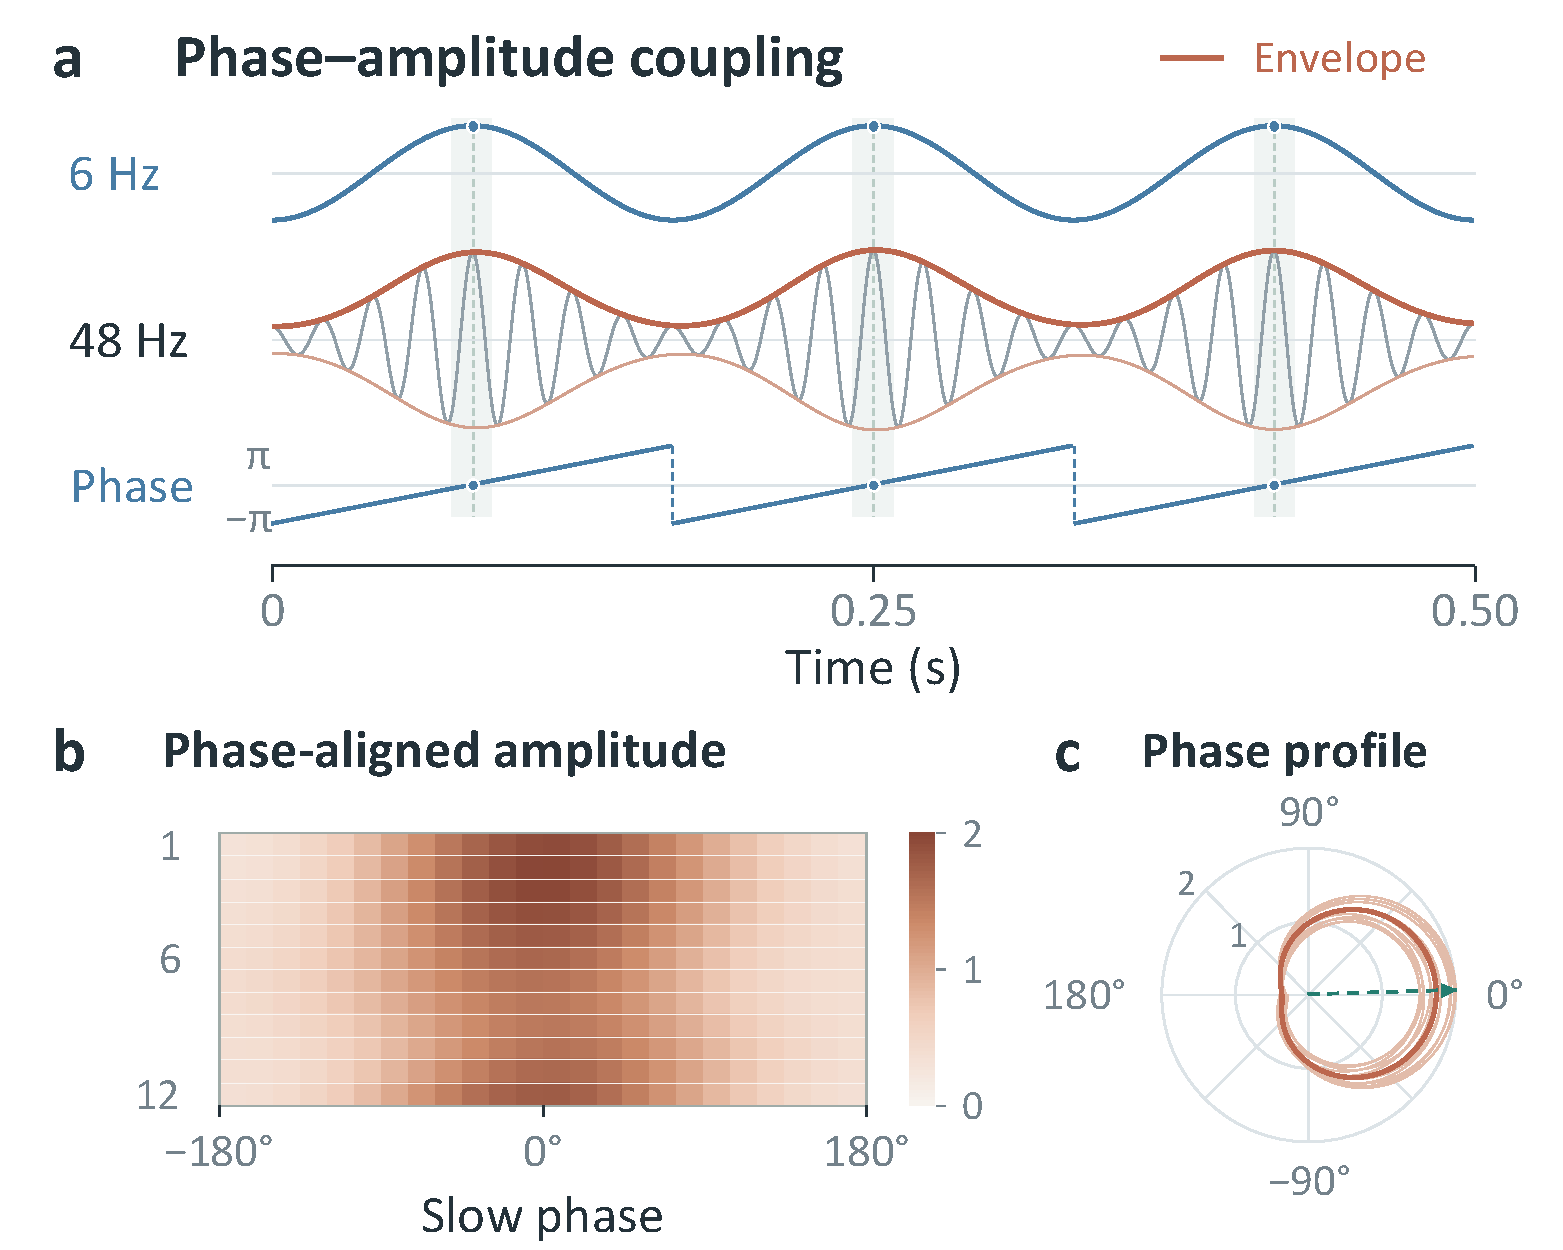
\includegraphics[width=\linewidth]{figures/pac_intro_inset.pdf}
\caption{\textbf{PAC intuition.} Illustrative signals: (a) a fast rhythm's envelope varies with slow phase; (b) phase-aligned envelopes; (c) polar profiles reveal the preferred phase.}
\label{fig:pac-intuition}
\vspace{-8pt}
\end{wrapfigure}
A tokenizer determines which EEG structure an encoder receives explicitly.
Common designs encode waveform patches, spectral patches, or their
combination \citep{yang2023biot,jiang2024labram,wang2025cbramod}, leaving
relations between bands to downstream learning. We ask whether a measured
cross-band relation should instead determine how a token is constructed.

Phase--amplitude coupling (PAC) provides the organizing principle: a
slower rhythm's phase is associated with variation in a faster rhythm's
amplitude. It is studied in cortical activity, seizures and sleep
\citep{canolty2006high,amiri2016phase,staresina2015hierarchical}. We translate
this principle into a computational prior, without treating our short-window
statistic as a validated physiological PAC measurement.

\begin{figure}[!t]
\centering
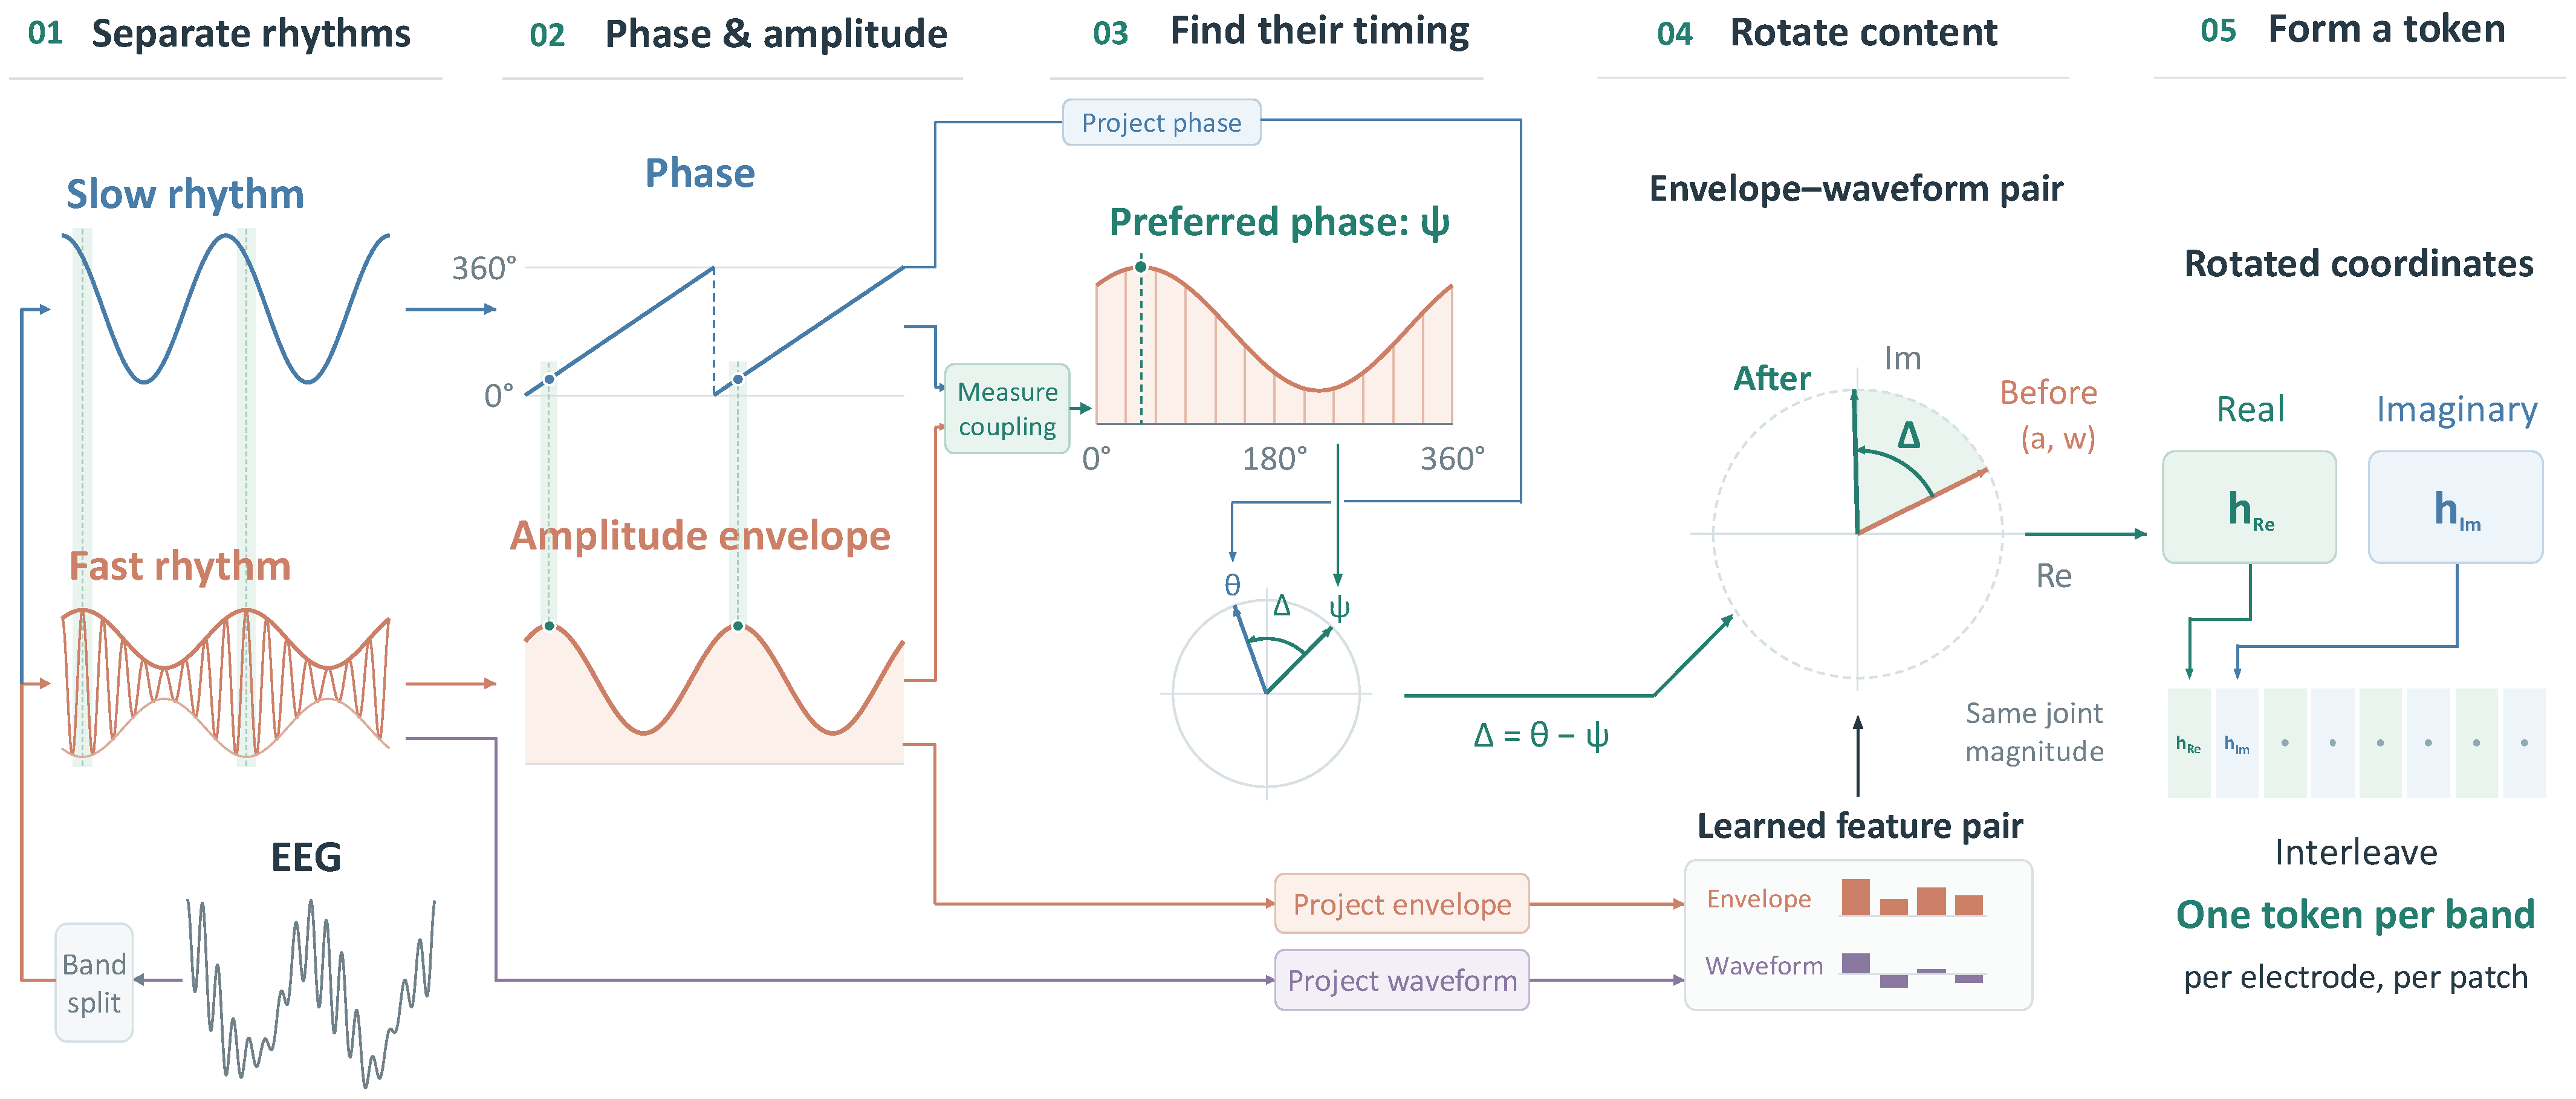
\includegraphics[width=\textwidth]{figures/crofremo_fig1_symbolic.pdf}
\caption{\textbf{From cross-frequency timing to a token.} Schematic with one source band and one feature pair. Separate rhythms, extract phase and envelope, and estimate a preferred phase $\psi$. The relative direction $\Delta=\theta-\psi$ rotates the envelope--waveform pair $(a,w)$ while preserving its joint magnitude. Real and imaginary coordinates are interleaved into a token; the full operator combines multiple sources.}
\label{fig:algorithm}
\end{figure}
\textbf{CroFreMo (Cross-Frequency Modulation)} uses a learned filterbank
and local complex phase--amplitude moments. Moment magnitudes weight source
bands; their angles align projected phase features into a direction that
rotates target-band content. A real envelope coordinate and an imaginary
waveform coordinate retain complementary content in one row per band.
The relation defines the token's coordinate frame rather than an extra
feature appended to an otherwise unchanged representation.

The main test holds the frontend grid and encoder fixed while replacing
measured alignment with identity, own phase, or magnitude weighting, and
while removing waveform content. Native-grid adapters then test reuse in
BIOT and CBraMod. Our contributions are:
\begin{itemize}[leftmargin=*,itemsep=2pt,topsep=2pt]
\item A \textbf{cross-frequency tokenization operator} that converts measured
phase--amplitude relations into content coordinates.
\item \textbf{Component and identity controls} that distinguish alignment,
weighting and waveform content, with task-dependent effects.
\item A \textbf{compact reference model and reusable frontend}: 1.22M
parameters achieve competitive benchmark results, with adapter experiments
in BIOT and CBraMod \citep{yang2023biot,wang2025cbramod}.
\end{itemize}

\section{Related Work}
\label{sec:related}
\paragraph{EEG foundation models and tokenization.}
EEGNet and EEG Conformer exemplify compact supervised EEG architectures
\citep{lawhern2018eegnet,song2023eeg}. Foundation models extend this setting
through self-supervised objectives: BENDR uses contrastive learning;
MAEEG, BrainBERT, EEG2Rep and EEGPT reconstruct or predict latent
representations \citep{kostas2021bendr,chien2022maeeg,wang2023brainbert,foumani2024eeg2rep,wang2024eegpt}.
Neuro-GPT and NeuroLM study generative interfaces
\citep{cui2024neurogpt,jiang2025neurolm}, while montage-aware representations
address heterogeneous electrodes \citep{yi2023learning,elouahidi2025reve,doner2025luna}.
At the input, BIOT embeds spectra, LaBraM learns neural codes, and CBraMod
combines temporal and spectral features
\citep{yang2023biot,jiang2024labram,wang2025cbramod}. TFM-Tokenizer and
CodeBrain make time--frequency tokenization central
\citep{pradeepkumar2026tfm,ma2026codebrain}. CroFreMo's distinction is the
use of a measured cross-band relation to set feature coordinates.

\paragraph{Phase--amplitude organization as a prior.}
Modulation is studied in natural-sound representations
\citep{singh2003modulation} and in neural coordination and memory
\citep{jensen2007cross,canolty2010functional,lisman2013theta,hyafil2015neural}.
Clinical studies examine seizure activity, sleep nesting, Parkinson disease,
anesthesia and dementia
\citep{edakawa2016detection,staresina2015hierarchical,dehemptinne2013exaggerated,purdon2013electroencephalogram,goodman2018theta}.
PAC estimators address phase clustering and event-related structure
\citep{tort2010measuring,voytek2013method,vandriel2015phase}, with known
confounds from nonstationarity and waveform shape
\citep{aru2015untangling,cole2017brain}. SleepPACNet and FAPEX introduce
PAC-derived information into predictive networks
\citep{lee2026sleeppacnet,zheng2025fapex}. We study a coordinate construction
inspired by that literature, not a replacement physiological estimator.

\section{Method}
\label{sec:method}

CroFreMo decomposes EEG into bands, measures local relations, aligns
source phases and rotates content before encoding (Figure~\ref{fig:architecture}).

\subsection{Patch-level phase--amplitude geometry}
\label{sec:phenomenon}
Let $x\in\mathbb{R}^{C\times T}$ be an EEG window sampled at $f_s$. A
learnable sinc filterbank \citep{ravanelli2018sincnet}, initialized on a
logarithmic grid over 0.5--75 Hz (0.5--49 Hz for 100-Hz Sleep-EDF, to
stay below Nyquist), produces $n_b$ band signals $x_b(t)$. The analytic
signal $z_b=x_b+i\mathcal{H}[x_b]$ of each band splits it into an
envelope $A_b=|z_b|$ and a unit phase $p_b=e^{i\phi_b}$, computed in the
implementation as $z_b/\max(A_b,10^{-6})$. Filtering and the Hilbert
transform run over the whole window (5\,s on TUEV) before any patching;
the patch only sets the interval over which the moment below is
averaged.

PAC is the dependence of a fast band's amplitude $A_j$ on a slow band's
phase $\phi_i$ \citep{canolty2006high,tort2010measuring}. We use its phase--amplitude organization principle through a centered
first circular moment inside each electrode and estimation window
\citep{voytek2013method,vandriel2015phase}:
\begin{equation}
Z_{ij} \;=\; \frac{c_Z}{\ell}\sum_{t\in\text{patch}}
p_i(t)\bigl(A_j(t)-\bar A_j\bigr).
\label{eq:mvl}
\end{equation}
$c_Z=10^{-2}$ is a numerical scale; the alignment below normalizes it
away everywhere except at the guards. Centering removes the mean-envelope contribution under nonuniform phase
sampling. The complex moment retains both relative magnitude and
preferred-phase information. Pairs are
taken as $i<j$ in band-index order. The cutoffs start in increasing
frequency order and training is free to move them, so $i<j$ is an index
convention rather than a guarantee that every pair is slow-to-fast.





Short token patches retain local waveform detail for transient-event
classification, whereas slow phase--amplitude relations may require longer
estimation windows. We separate these time scales: token patches remain
50 samples (0.25\,s at 200\,Hz; 0.5\,s on Sleep-EDF), while the moment
window can span multiple patches. The reference uses $\ell=50$ for both;
host adapters pool tokens to their native grid. This resolution is a
design choice, not an established optimum. Below 4\,Hz, a 0.25-s window
contains less than one cycle, so $Z_{ij}$ is local phase-weighted amplitude
covariance, not a cycle-averaged physiological PAC estimate. Non-stationarity
and waveform shape can also affect it \citep{aru2015untangling,cole2017brain}.
Appendix~\ref{app:band-mixer} varies estimation context while holding
token resolution fixed on the band-mixer encoder.

\subsection{PAC-inspired cross-frequency modulation}
\label{sec:tokenizer}
Each band and patch yields three learned features: a waveform feature
$\mathbf w_b=L_w(x_b[\mathrm{patch}])\in\mathbb R^{d/2}$, a log-envelope
feature $\mathbf a_b=\mathbf s_a\odot L_a(\log(1+A_b[\mathrm{patch}]))
\in\mathbb R^{d/2}$, and a complex phase feature
$\tilde{\mathbf p}_b=L_p(p_b[\mathrm{patch}])\in\mathbb C^{d/2}$. $L_w$
is bias-free and starts at zero; $L_a$ is affine, with a learned diagonal
calibration $\mathbf s_a$ initialized to one; $L_p$ applies one real,
bias-free map to the real and imaginary parts alike and is therefore
complex-linear, a property the invariance below depends on.

The moment decides how eligible source-phase features are combined for
band $j$:
\begin{equation}
\mathbf u_j=\sum_{i<j}\alpha_{ij}\eta_{ij}
\tilde{\mathbf p}_i,\qquad
\alpha_{ij}=\frac{|Z_{ij}|}{\sum_{i'<j}|Z_{i'j}|}.
\label{eq:aligned}
\end{equation}
Here $\eta_{ij}=Z_{ij}^*/\max(|Z_{ij}|,\epsilon_w)$ with
$\epsilon_w=10^{-8}$, which away from the guard is just
$e^{-i\angle Z_{ij}}$: each slow band's phase feature is rotated back by
the preferred phase measured against band $j$; larger relative moment
magnitudes receive larger weights. The first indexed band has no eligible source
and keeps its own phase, $\mathbf u_0=\tilde{\mathbf p}_0$. A column whose
magnitudes sum to at most $\epsilon_w$ falls back to a plain average of
the lower bands' phase features.

\begin{proposition}[Phase-reference invariance]
\label{prop:invariance}
For $j>0$ outside the fallback regime, $\mathbf u_j$ is invariant to
independent reference changes $p_i\mapsto e^{i\delta_i}p_i$ in the
analytic representation.
\end{proposition}
A change of phase reference multiplies $\tilde{\mathbf p}_i$ and $Z_{ij}$
by the same factor, and $\eta_{ij}$ undoes it. This is why coupling
enters through the aligned phase and not through the raw phases: the
raw phase of a band depends on the analysis convention, whereas the
aligned phase is invariant to the specified reference change. This
is not invariance to an arbitrary waveform perturbation. Proofs are in
Appendix~\ref{app:modulation-properties}.

The modulation token rotates the joint envelope--waveform feature by the
normalized alignment:
\begin{equation}
\mathbf q_j=\mathbf a_j+i\mathbf w_j,\qquad
\mathbf h_j=\mathbf q_j\odot
\frac{\mathbf u_j}{\max(|\mathbf u_j|,\epsilon)},\qquad
\epsilon=10^{-6}.
\label{eq:rotation}
\end{equation}
For $|u|\ge\epsilon$, each coordinate pair preserves $|h|^2=a^2+w^2$;
below the guard it is attenuated (Appendix~\ref{app:modulation-properties}).





Above the normalization guard, the coupling changes feature direction
without changing the joint envelope--waveform magnitude. Normalization
separates coordinate alignment from amplitude rescaling. It also removes
absolute coupling confidence: relative weights survive, but a globally
weak moment can still induce a full rotation. Shuffled-moment controls
probe input--relation correspondence; they do not certify physiological
coupling or reliability under weak moments.

\begin{figure}[!t]
\centering
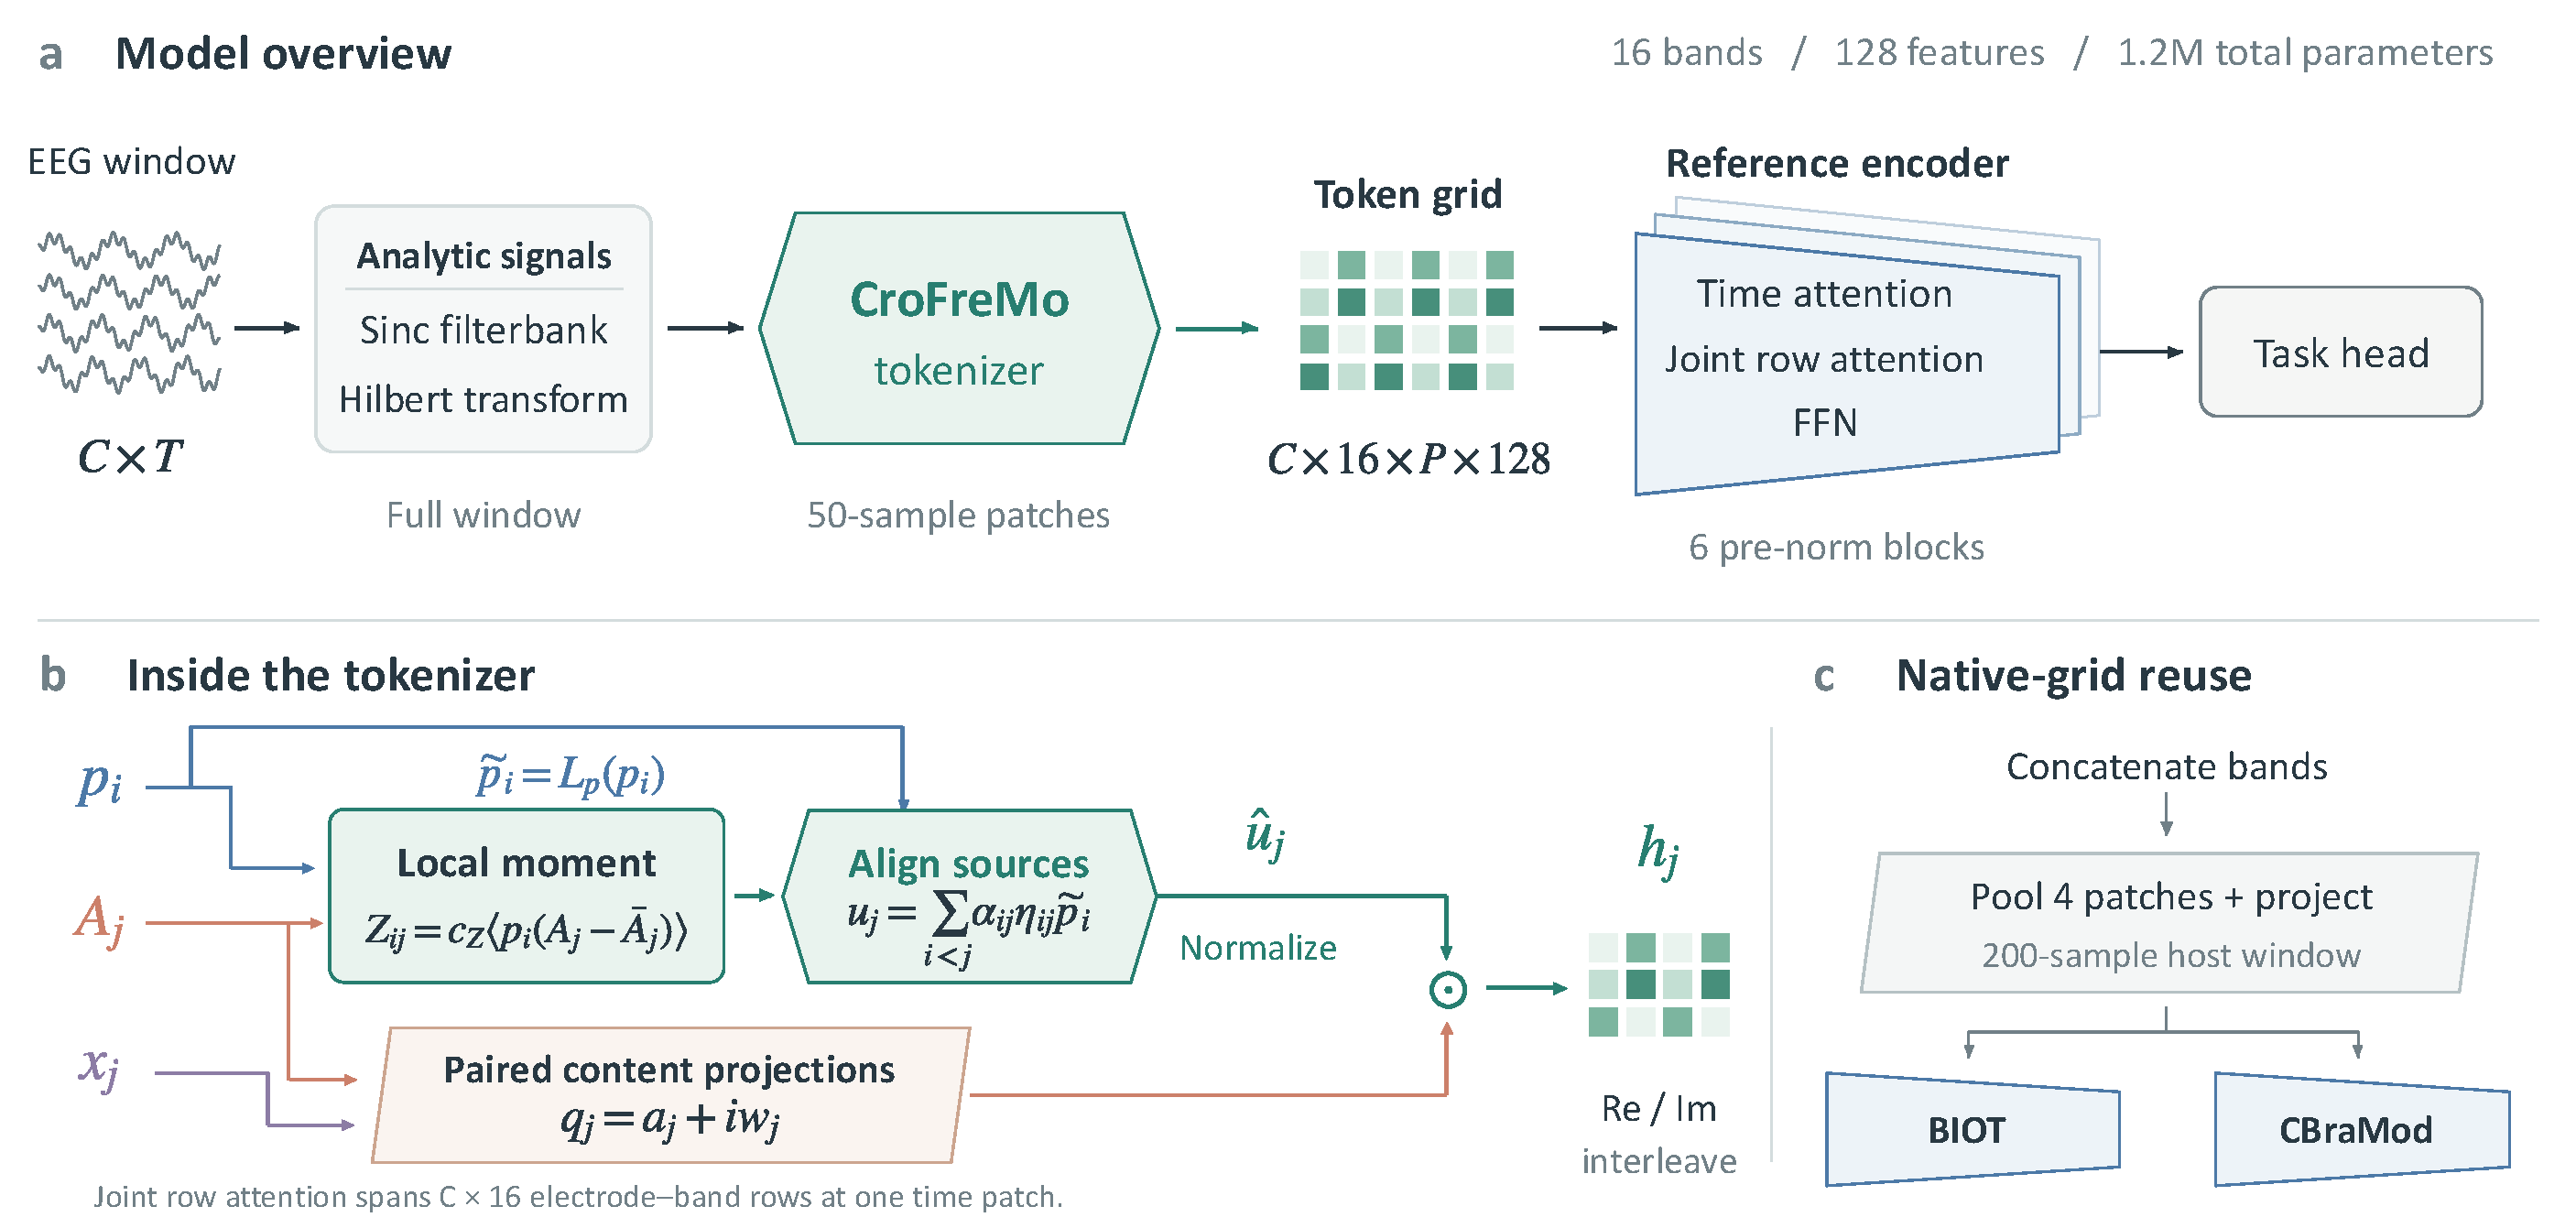
\includegraphics[width=\textwidth]{figures/crofremo_v2_architecture.pdf}
\caption{\textbf{CroFreMo: architecture, token construction, and reuse.} (a) Full-window analytic signals feed a 16-band tokenizer and six two-axis encoder blocks, with attention along time and joint electrode--band rows. (b) Local phase--amplitude moments align source phases; the normalized direction rotates paired envelope and waveform features before real/imaginary interleaving. (c) Band concatenation, patch pooling, and projection adapt the tokens to BIOT or CBraMod.}


\label{fig:architecture}\label{fig:pretraining}
\end{figure}

The rotation differs from rotary position embeddings, whose angles encode
position \citep{su2024roformer}, and from feature-wise affine conditioning
\citep{perez2018film}: here its direction is computed from the input's
cross-band moment. This distinction specifies the construction; superiority
over PAC-as-feature conditioning requires a separate controlled comparison.

\subsection{Complementary content in one token}
\label{sec:waveform-complement}
The envelope omits waveform sign and shape. CroFreMo retains them in the
imaginary coordinate and rotates the feature pair together.
With $\widehat u=\cos\theta+i\sin\theta$, each feature pair transforms as
\begin{equation}
\begin{bmatrix}\operatorname{Re}h\\\operatorname{Im}h\end{bmatrix}
=\begin{bmatrix}\cos\theta&-\sin\theta\\\sin\theta&\cos\theta\end{bmatrix}
\begin{bmatrix}a\\w\end{bmatrix}.
\label{eq:quadrature}
\end{equation}
Real and imaginary coordinates are interleaved into one token per band.
Since $L_w$ starts at zero, waveform content is learned from an
envelope-only initialization.



\subsection{Reference encoder}
\label{sec:encoder}
Tokens form a $C\times n_b\times P\times d$ grid processed by $N$
pre-norm transformer blocks \citep{vaswani2017attention}. Temporal
attention operates along each electrode--band row, with rotary positions
\citep{su2024roformer}. Joint row attention then mixes all $C n_b$ rows
at each patch, followed by a feed-forward layer. Learned band-index and
spatial embeddings identify rows. The reference uses $n_b=16$, $d=128$,
$N=6$, and four heads, totaling 1.22M parameters in the TUEV configuration.
It has no separate band-only attention sub-layer, but joint row attention
can still learn cross-band interactions. The controls therefore test the
benefit of explicit token construction, not whether an encoder is incapable
of learning cross-frequency structure. An alternative three-axis encoder
with a band-only sub-layer is reported in Appendix~\ref{app:band-mixer}.

\subsection{Integration with existing encoders}
\label{sec:quad-pretrain}
To put the tokenizer inside an encoder we did not design
(Figure~\ref{fig:architecture}c), we concatenate the sixteen band tokens,
average four 50-sample patches into each 200-sample host window, and
project to the host's width (200 for CBraMod, 256 for BIOT). The host-specific encoder, positional modules and classifier are retained
\citep{yang2023biot,wang2025cbramod}; native and replacement frontends are
compared using the recorded host recipes. The host
therefore sees its usual token grid filled with our tokens, while the matched identity variant isolates modulation within the
replacement frontend.
The host encoders are trained from scratch; the separate TFM-Tokenizer
comparison uses a frozen pretrained codebook. This is a test of whether the
frontend transfers, not of compatibility with released pretrained
weights; the matched identity frontend in
Section~\ref{sec:transplant} separates the coupling from the rest of the
frontend.

% --- setup ---
\section{Experimental Setup}
\label{sec:setup}
\paragraph{Datasets and training.}
The ten reported corpora span events, seizure detection, artifacts,
diagnosis and sleep staging \citep{obeid2016temple,shoeb2009application,jing2023development,kemp2000analysis,khalighi2016isruc}.
Appendix~\ref{app:corpora-details} describes preprocessing and splits.
CroFreMo uses 16 bands, width 128, six two-axis blocks, four heads, and
50-sample patches. The filterbank is initialized over 0.5--75 Hz at 200 Hz
to cover the usable preprocessing passband. On 100-Hz Sleep-EDF, the range
is 0.5--49 Hz to respect Nyquist at initialization; the upper cutoff is clamped during training.
AdamW \citep{loshchilov2019decoupled} uses learning rate $10^{-4}$, weight decay 0.05, dropout 0.35,
batch size 32, cosine decay, and gradient clipping at 1.0.
Losses, validation cadence, and stopping rules are dataset-specific.
One configured augmentation is sampled per training forward pass.

\paragraph{Evaluation.}
Runs use seeds 0, 1 and 2; within each run the checkpoint is chosen on
the validation split and the test split is scored once. Entries with
$\pm$ are mean and sample SD over three seeds unless a smaller count is stated; entries without a
spread are single runs. Bold marks the best value in a column. Primary metrics are AUC-PR
(trapezoidal) for TUSZ and CHB-MIT, balanced accuracy for TUAB and ADFD, AUROC for TUEP, and Cohen's $\kappa$ elsewhere. Dashes are cells
we have not run. Model size counts trainable parameters, classifier included, at the TUEV configuration (16 channels, 5\,s); a head that
flattens the token grid, as CBraMod's does, grows with the input shape.

\paragraph{Baselines.}
We compare supervised models, released-pretrained models, and foundation
architectures trained from scratch
\citep{lawhern2018eegnet,song2023eeg,yang2023biot,jiang2024labram,wang2025cbramod,wang2024eegpt,pradeepkumar2026tfm,elouahidi2025reve}.
The supervised and from-scratch groups are the closest comparisons.
Released-weight rows retain recorded adaptation pipelines and can differ
in preprocessing and processed examples. Rankings are descriptive;
they neither isolate pretraining nor imply uniformly matched tuning
budgets (Appendix~\ref{app:comparison-scope}).

% --- results ---



% --- main baselines ---
% --- single tuev iiic ---
\begin{table}[!t]
\centering
\caption{Benchmark results on TUEV and IIIC.}
\label{tab:baseline-tuev}
\label{tab:baseline-iiic}
\TableStyle\fontsize{7.5}{8.3}\selectfont\renewcommand{\arraystretch}{0.95}\setlength{\aboverulesep}{1pt}\setlength{\belowrulesep}{1pt}
\begin{tabular*}{\textwidth}{@{\extracolsep{\fill}}lccccccc@{}}
\toprule
Method & Size & \multicolumn{3}{c}{TUEV} & \multicolumn{3}{c}{IIIC} \\
\midrule
 & (M) & Bal. acc. & $\kappa$ & W-F1 & Bal. acc. & $\kappa$ & W-F1 \\
\midrule
\multicolumn{8}{l}{\textit{Supervised}} \\
SPaRCNet & 0.99 & $0.465\!\pm\!0.035$ & $0.488\!\pm\!0.028$ & $0.735\!\pm\!0.015$ & $0.477\!\pm\!0.010$ & $0.372\!\pm\!0.012$ & $0.479\!\pm\!0.011$ \\
CNN-Transformer & 3.16 & $0.368\!\pm\!0.103$ & $0.410\!\pm\!0.116$ & $0.692\!\pm\!0.074$ & $0.515\!\pm\!0.008$ & $0.416\!\pm\!0.009$ & $0.513\!\pm\!0.014$ \\
FFCL & 2.42 & $0.438\!\pm\!0.069$ & $0.478\!\pm\!0.032$ & $0.737\!\pm\!0.017$ & $0.520\!\pm\!0.018$ & $0.423\!\pm\!0.020$ & $0.524\!\pm\!0.017$ \\
ST-Transformer & 3.43 & $0.473\!\pm\!0.020$ & $0.501\!\pm\!0.012$ & $0.741\!\pm\!0.009$ & $0.407\!\pm\!0.002$ & $0.296\!\pm\!0.002$ & $0.408\!\pm\!0.008$ \\
EEGNet & $<$0.01 & $0.415\!\pm\!0.057$ & $0.479\!\pm\!0.091$ & $0.739\!\pm\!0.037$ & $0.298\!\pm\!0.013$ & $0.109\!\pm\!0.009$ & $0.131\!\pm\!0.015$ \\
EEGConformer & 0.78 & $0.421\!\pm\!0.045$ & $0.455\!\pm\!0.004$ & $0.717\!\pm\!0.006$ & $0.362\!\pm\!0.012$ & $0.189\!\pm\!0.018$ & $0.268\!\pm\!0.004$ \\
\midrule
\multicolumn{8}{l}{\textit{Released pretrained}} \\
BIOT & 3.19 & $0.489\!\pm\!0.030$ & $0.530\!\pm\!0.028$ & $0.753\!\pm\!0.016$ & $0.465\!\pm\!0.015$ & $0.361\!\pm\!0.016$ & $0.466\!\pm\!0.013$ \\
LaBraM & 5.82 & $0.630\!\pm\!0.031$ & $0.598\!\pm\!0.003$ & $0.809\!\pm\!0.005$ & $0.483\!\pm\!0.018$ & $0.383\!\pm\!0.020$ & $0.485\!\pm\!0.019$ \\
CBraMod & 17.9 & $0.603\!\pm\!0.011$ & $0.645\!\pm\!0.022$ & $0.813\!\pm\!0.012$ & $0.416\!\pm\!0.015$ & $0.313\!\pm\!0.019$ & $0.418\!\pm\!0.018$ \\
EEGPT & 25.7 & $0.513\!\pm\!0.075$ & $0.574\!\pm\!0.040$ & $0.777\!\pm\!0.020$ & $0.497\!\pm\!0.018$ & $0.397\!\pm\!0.019$ & $0.500\!\pm\!0.014$ \\
TFM-Tokenizer & 1.89 & $0.596\!\pm\!0.036$ & $0.652\!\pm\!0.021$ & $0.817\!\pm\!0.010$ & $0.506\!\pm\!0.009$ & $0.406\!\pm\!0.009$ & $0.508\!\pm\!0.007$ \\
REVE & 69.5 & $0.648\!\pm\!0.018$ & $0.685\!\pm\!0.039$ & $0.838\!\pm\!0.019$ & $0.529\!\pm\!0.003$ & $0.436\!\pm\!0.003$ & $0.534\!\pm\!0.003$ \\
\midrule
\multicolumn{8}{l}{\textit{From scratch}} \\
BIOT & 3.19 & $0.535\!\pm\!0.062$ & $0.532\!\pm\!0.025$ & $0.761\!\pm\!0.013$ & $0.460\!\pm\!0.014$ & $0.356\!\pm\!0.014$ & $0.462\!\pm\!0.015$ \\
LaBraM & 5.82 & $0.372\!\pm\!0.085$ & $0.372\!\pm\!0.009$ & $0.693\!\pm\!0.013$ & $0.505\!\pm\!0.005$ & $0.406\!\pm\!0.007$ & $0.504\!\pm\!0.006$ \\
CBraMod & 17.9 & $0.574\!\pm\!0.010$ & $0.564\!\pm\!0.024$ & $0.767\!\pm\!0.004$ & $0.489\!\pm\!0.005$ & $0.393\!\pm\!0.006$ & $0.497\!\pm\!0.004$ \\
EEGPT & 25.7 & $0.449\!\pm\!0.036$ & $0.556\!\pm\!0.012$ & $0.765\!\pm\!0.011$ & $0.472\!\pm\!0.021$ & $0.368\!\pm\!0.024$ & $0.476\!\pm\!0.020$ \\
TFM-Tokenizer & 1.89 & $0.420\!\pm\!0.016$ & $0.582\!\pm\!0.020$ & $0.818\!\pm\!0.018$ & $0.385\!\pm\!0.006$ & $0.263\!\pm\!0.008$ & $0.381\!\pm\!0.009$ \\
\midrule
CroFreMo & 1.22 & $\mathbf{0.650}\!\pm\!0.035$ & $\mathbf{0.711}\!\pm\!0.014$ & $\mathbf{0.851}\!\pm\!0.008$ & $\mathbf{0.548}\!\pm\!0.021$ & $\mathbf{0.469}\!\pm\!0.013$ & $\mathbf{0.555}\!\pm\!0.019$ \\
\bottomrule
\end{tabular*}
\vspace{5pt}
\centering
\caption{Benchmark results on TUSZ and CHB-MIT. Checkpoints are validation-selected; spreads denote sample SD. Training budgets and pipeline differences are discussed in the text.}
\label{tab:baseline-tusz}
\label{tab:baseline-chbmit}
\TableStyle\fontsize{7.5}{8.3}\selectfont\renewcommand{\arraystretch}{0.95}\setlength{\aboverulesep}{1pt}\setlength{\belowrulesep}{1pt}
\begin{tabular*}{\textwidth}{@{\extracolsep{\fill}}lccccccc@{}}
\toprule
Method & Size & \multicolumn{3}{c}{TUSZ} & \multicolumn{3}{c}{CHB-MIT} \\
\midrule
 & (M) & Bal. acc. & AUC-PR & AUROC & Bal. acc. & AUC-PR & AUROC \\
\midrule
\multicolumn{8}{l}{\textit{Supervised}} \\
SPaRCNet & 0.99 & $0.561\!\pm\!0.038$ & $0.502\!\pm\!0.021$ & $0.889\!\pm\!0.002$ & $0.513\!\pm\!0.008$ & $0.198\!\pm\!0.071$ & $0.799\!\pm\!0.037$ \\
CNN-Transformer & 3.16 & $0.539\!\pm\!0.055$ & $0.371\!\pm\!0.193$ & $0.846\!\pm\!0.042$ & $0.642\!\pm\!0.058$ & $0.506\!\pm\!0.074$ & $0.911\!\pm\!0.008$ \\
FFCL & 2.42 & $0.595\!\pm\!0.033$ & $0.545\!\pm\!0.030$ & $0.892\!\pm\!0.011$ & $0.616\!\pm\!0.015$ & $0.534\!\pm\!0.054$ & $0.912\!\pm\!0.011$ \\
ST-Transformer & 3.43 & $0.551\!\pm\!0.042$ & $0.359\!\pm\!0.031$ & $0.815\!\pm\!0.020$ & $0.555\!\pm\!0.104$ & $0.241\!\pm\!0.113$ & $0.721\!\pm\!0.104$ \\
EEGNet & $<$0.01 & $0.521\!\pm\!0.011$ & $0.492\!\pm\!0.030$ & $0.873\!\pm\!0.004$ & $0.602\!\pm\!0.146$ & $0.141\!\pm\!0.135$ & $0.744\!\pm\!0.110$ \\
EEGConformer & 0.78 & $0.522\!\pm\!0.037$ & $0.319\!\pm\!0.038$ & $0.819\!\pm\!0.028$ & $0.500\!\pm\!0.000$ & $0.305\!\pm\!0.253$ & $0.597\!\pm\!0.168$ \\
\midrule
\multicolumn{8}{l}{\textit{Released pretrained}} \\
BIOT & 3.19 & $0.563\!\pm\!0.033$ & $0.338\!\pm\!0.038$ & $0.838\!\pm\!0.014$ & $0.619\!\pm\!0.045$ & $0.560\!\pm\!0.077$ & $0.874\!\pm\!0.004$ \\
LaBraM & 5.82 & $0.614\!\pm\!0.038$ & $0.475\!\pm\!0.047$ & $0.869\!\pm\!0.025$ & $0.586\!\pm\!0.047$ & $0.452\!\pm\!0.097$ & $0.871\!\pm\!0.062$ \\
CBraMod & 17.9 & $0.635\!\pm\!0.034$ & $0.434\!\pm\!0.042$ & $0.852\!\pm\!0.005$ & $0.545\!\pm\!0.020$ & $0.233\!\pm\!0.098$ & $0.783\!\pm\!0.047$ \\
EEGPT & 25.7 & $0.659\!\pm\!0.062$ & $0.545\!\pm\!0.070$ & $0.882\!\pm\!0.012$ & $0.547\!\pm\!0.063$ & $0.281\!\pm\!0.133$ & $0.857\!\pm\!0.038$ \\
TFM-Tokenizer & 1.89 & $0.564\!\pm\!0.027$ & $0.347\!\pm\!0.018$ & $0.829\!\pm\!0.006$ & $0.634\!\pm\!0.016$ & $0.627\!\pm\!0.025$ & $0.929\!\pm\!0.006$ \\
REVE & 69.5 & $0.552\!\pm\!0.037$ & $0.503\!\pm\!0.075$ & $0.889\!\pm\!0.016$ & $0.632\!\pm\!0.068$ & $0.580\!\pm\!0.196$ & $0.898\!\pm\!0.064$ \\
\midrule
\multicolumn{8}{l}{\textit{From scratch}} \\
BIOT & 3.19 & $0.616\!\pm\!0.065$ & $0.347\!\pm\!0.026$ & $0.826\!\pm\!0.017$ & $0.624\!\pm\!0.071$ & $0.566\!\pm\!0.072$ & $0.875\!\pm\!0.019$ \\
LaBraM & 5.82 & $0.581\!\pm\!0.036$ & $0.475\!\pm\!0.048$ & $0.858\!\pm\!0.019$ & $0.585\!\pm\!0.065$ & $0.360\!\pm\!0.050$ & $0.823\!\pm\!0.030$ \\
CBraMod & 17.9 & $0.576\!\pm\!0.049$ & $0.482\!\pm\!0.052$ & $0.875\!\pm\!0.033$ & $0.602\!\pm\!0.088$ & $0.317\!\pm\!0.205$ & $0.780\!\pm\!0.133$ \\
\midrule
CroFreMo & 1.22 & $\mathbf{0.664}\!\pm\!0.033$ & $\mathbf{0.650}\!\pm\!0.045$ & $\mathbf{0.915}\!\pm\!0.051$ & $\mathbf{0.664}\pm0.023$ & $\mathbf{0.690}\pm0.017$ & $\mathbf{0.931}\pm0.008$ \\
\bottomrule
\end{tabular*}
\par\vspace{3pt}{\TableFont Bold: best displayed value per column (ties included). Size: trainable parameters (M) at the TUEV configuration.}
\end{table}
\section{Results}
\label{sec:results}
\subsection{Predictive performance across tasks}
\label{sec:main}
Tables~\ref{tab:baseline-tuev} and~\ref{tab:baseline-tusz} summarize four
clinical EEG tasks; six further corpora appear in Appendix~\ref{app:matrix}.
CroFreMo has the highest displayed mean in all six columns of each main
table. On TUEV, $\kappa=0.711\pm0.014$ compares with $0.685\pm0.039$ for
REVE \citep{elouahidi2025reve}. On IIIC it reaches $0.469\pm0.013$.
For seizure detection, AUC-PR is $0.650\pm0.045$ on TUSZ and
$0.690\pm0.017$ on CHB-MIT; the highest baseline means are 0.545 and
0.627, respectively, the latter from TFM-Tokenizer
\citep{pradeepkumar2026tfm}. These are descriptive comparisons of the
reported means, not significance tests.

The broader benchmark shows where the advantage narrows. CroFreMo reaches
$\kappa=0.704\pm0.015$ on TUAR, 0.684 on Sleep-EDF, and
$0.770\pm0.008$ on ISRUC. It trails the best displayed primary metric on
TUAB, TUEP and ADFD. At 1.22M parameters, it is approximately 15 times
smaller than the evaluated CBraMod configuration and 57 times smaller than
REVE \citep{wang2025cbramod,elouahidi2025reve}. This is a parameter-count
advantage, not a measured throughput or memory advantage: the explicit
band grid increases token count. Appendix~\ref{app:complexity} gives the
corresponding scaling analysis.

% Exploratory eight-band comparisons remain in the appendix; the main
% evidence concerns controls within the final tokenizer architecture.


\subsection{Does measured alignment contribute?}
\label{sec:content-structure}
% --- main alignment ---
To distinguish the operator from the band grid and frontend, we retain
the reference architecture and vary its construction: identity removes
rotation; own phase uses each band's phase; weights only keeps
$\alpha$ but sets $\eta=1$; envelope only removes waveform content.
Figure~\ref{fig:main-alignment} summarizes all five variants;
Appendix~\ref{app:control-definition} gives their exact definitions.

\begin{figure}[!htbp]
\centering
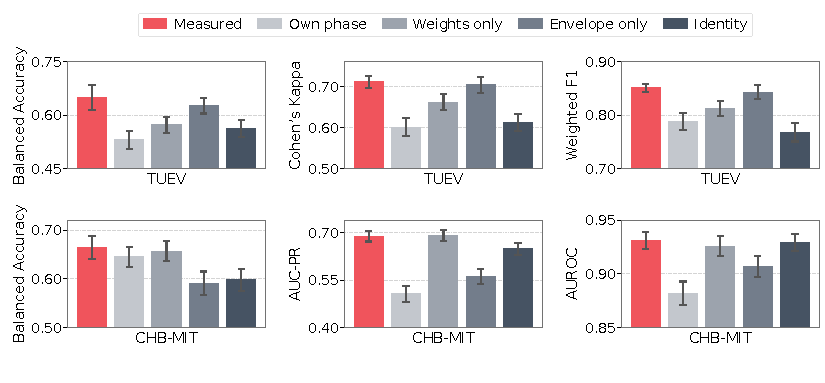
\includegraphics[width=\textwidth]{figures/table3_controls.pdf}
\caption{\textbf{Component controls for the two-axis CroFreMo tokenizer.} Bars show reported means; error bars show reported SD. Each row compares five variants on three metrics. Vertical axes are truncated. CHB-MIT arms have different training lengths and stopping conditions, so their ordering is not an equal-budget comparison.}
\label{fig:main-alignment}
\end{figure}



\paragraph{Alignment versus unrotated content.}
Identity is the direct no-rotation control. In Figure~\ref{fig:main-alignment},
measured alignment reaches mean TUEV $\kappa=0.711$, compared with 0.612
for identity; balanced accuracy is 0.650 versus 0.564. On CHB-MIT,
AUC-PR is 0.690 versus 0.650, but AUROC is close (0.931 versus 0.929).
The aggregate differences favor measured alignment on these metrics;
they do not establish a uniform gain across encoders, seeds or budgets.
The alternative band-mixer encoder has a different pattern: its TUEV
seed-0 identity control exceeds measured $\kappa$
(Appendix~\ref{app:band-mixer}). Removing a dedicated attention sub-layer
therefore does not, by itself, prove how either encoder uses the relation.

\paragraph{Separating angle, weighting and waveform content.}
On TUEV, replacing measured alignment with own phase, weights only, or
envelope only lowers mean $\kappa$ by 0.110, 0.049, and 0.007,
respectively. This ordering supports the alignment component within the
examined tokenizer. CHB-MIT differs: weights only reaches AUC-PR 0.692,
close to measured 0.690, whereas envelope only reaches 0.562 and own phase
0.507. Waveform retention is associated with a larger change on this
seizure task, but the unequal stopping conditions preclude an equal-budget
attribution. These task differences are consistent with heterogeneous EEG
features, rather than proof that a single physiological mechanism determines
all labels \citep{aru2015untangling,cole2017brain}.
The band-mixer shuffled-moment run reaches TUEV $\kappa=0.601$:
incorrect input--moment correspondence is detrimental in that experiment,
but shuffling also changes training noise. Full values and control
definitions appear in Appendices~\ref{app:display-values}
and~\ref{app:control-definition}.

\subsection{Reuse with existing EEG encoders}
\label{sec:transplant}

\begin{figure}[!htbp]
\centering
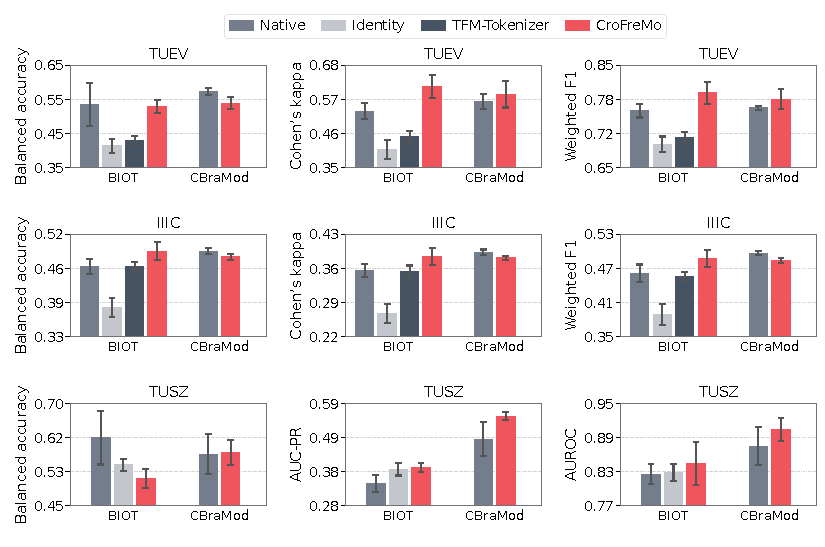
\includegraphics[width=\textwidth]{figures/host_reuse_bars.pdf}
\caption{\textbf{Encoder reuse.} Frontend comparisons within each host; bars and whiskers show reported means and SD. Identity removes modulation. TFM uses a frozen released codebook; its TUSZ result is unavailable. Axes are truncated. Full values and protocol details are in Appendix~\ref{app:display-values}.}
\label{fig:host-reuse}
\end{figure}






Figure~\ref{fig:host-reuse} tests replacement frontends in BIOT and CBraMod
\citep{yang2023biot,wang2025cbramod}. Within BIOT, measured and identity
share the replacement frontend, host and recipe; only modulation differs.
The recorded paired differences are $+0.201\pm0.007$ $\kappa$ on TUEV
and $+0.118\pm0.030$ on IIIC, positive in each of three seeds.
On TUSZ, the displayed AUC-PR means are close: 0.396 for measured and
0.391 for identity, compared with 0.347 for native BIOT. The
TFM-Tokenizer TUSZ replacement result is not available in this version.

Effects also depend on the host. Against native CBraMod, the recorded
paired $\kappa$ differences are $+0.023\pm0.020$ on TUEV and
$-0.012\pm0.007$ on IIIC; the TUSZ AUC-PR means are 0.552 and 0.482.
The frozen TFM-Tokenizer comparison \citep{pradeepkumar2026tfm} reaches
TUEV $\kappa=0.449\pm0.020$ and IIIC $0.354\pm0.012$ within BIOT.
It tests one released codebook and adapter, not every possible
implementation of feature-based tokenization. Earlier matched BIOT
CHB-MIT controls favor identity; Appendix~\ref{app:host-pairs} retains
that negative result. Thus architectural reuse is demonstrated, while
predictive gains remain host- and task-dependent. First-evaluation
validation peaks in the TUEV host runs are reported there as well.

\subsection{Inside the cross-frequency tokenizer}
\label{sec:inside-tokenizer}

\begin{figure}[!htbp]
\centering
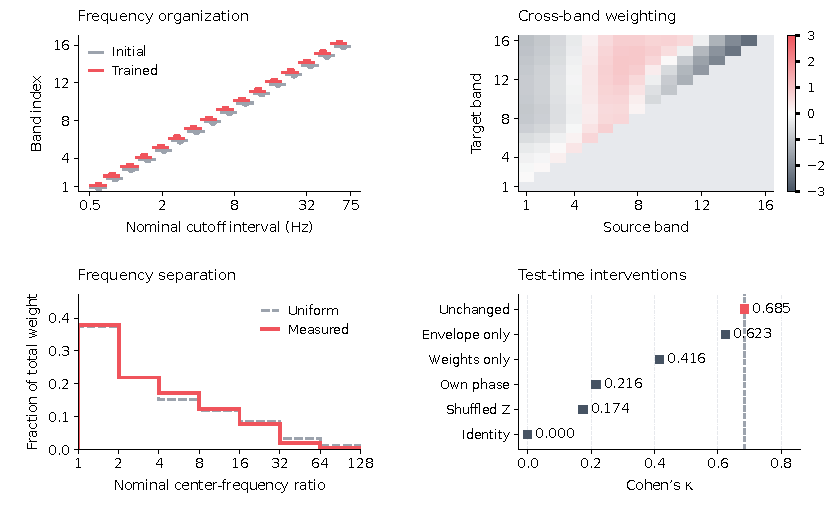
\includegraphics[width=\textwidth]{figures/tokenizer_diagnostics.pdf}
\caption{\textbf{Inside the two-axis tokenizer.} A fixed TUEV seed-0 checkpoint on all 29,421 test windows. Nominal filter intervals, weight enrichment over uniform sources, weight by frequency ratio, and inference interventions. The unchanged score is this checkpoint's value, not the main-table mean; interventions do not retrain the model.}
\label{fig:tokenizer-diagnostics}
\end{figure}

Figure~\ref{fig:tokenizer-diagnostics} analyzes the reference two-axis model
on all 29,421 TUEV test windows. The nominal band centers remain ordered,
but finite filter responses overlap at low frequencies. The ten largest
weight enrichments involve nominal frequency ratios 4.7--16.5 and
power-response overlaps below $5\times10^{-6}$. Across all 120 eligible
pairs, overlap and enrichment have Spearman $\rho=-0.02$.
This describes one checkpoint and does not eliminate other sources of
apparent coupling \citep{aru2015untangling}. In particular, total weight
in the ratio interval $[1,2)$ is 37.8\%, close to the 37.6\% uniform-source
reference; high enrichment and large total mass are different quantities.
Appendix~\ref{app:filter-overlap} gives the actual responses.

The unchanged checkpoint reproduces $\kappa=0.685$. At inference,
identity modulation gives 0.000, own phase 0.216, weights only 0.416,
shuffled moments 0.174, and envelope only 0.623. These changes show
sensitivity to the learned construction, not superiority over alternatives
retrained with it. The waveform pathway is active: per-band
$\operatorname{RMS}(w)/\operatorname{RMS}(a)$ ranges from 0.041 to 5.466.
Appendix~\ref{app:diagnostic-protocol} reports the intervention protocol,
class metrics, and the distinction from the aggregate main results.

\paragraph{Limitations.}
Small seed sets and unequal stopping budgets limit attribution; SD is not
a significance test. Native and shared loaders can differ in preprocessing,
and tuning budgets are not uniform across baselines. Local moments over
learned bands are PAC-inspired statistics, not validated physiological
measurements \citep{aru2015untangling}. Frequency order is not constrained,
and low-frequency filter responses can overlap. We do not establish an
advantage over a matched PAC-as-feature frontend, faster inference, or
successful CroFreMo pretraining. Host gains are task-dependent, including
negative CHB-MIT results. These boundaries distinguish an effective
representation design from a universal physiological or transfer claim.

\section{Conclusion}
CroFreMo uses local phase--amplitude relations to set the coordinates of
EEG content features before encoding. The 1.22M-parameter supervised
reference model is competitive across the benchmark, with the highest
displayed main-table means on TUEV, IIIC, TUSZ and CHB-MIT. Component
controls favor measured alignment over own-phase and identity on TUEV,
while CHB-MIT shows a stronger dependence on waveform content and a
smaller distinction between measured alignment and magnitude weighting.
BIOT and CBraMod experiments establish frontend reuse with task-dependent
predictive effects. The central contribution is an explicit cross-frequency
token construction; the compact reference architecture makes that design
practical to study without large-scale pretraining.

% The three statements below do NOT count toward the 9-page limit.
% "AI use statement" is REQUIRED by ICLR 2027; the other two are recommended.
% --- statements ---
% ---------------------------------------------------------------------------
% None of the three statements below counts toward the 9-page main-text limit
% (ICLR 2027 template, original lines 399/416/430). The AI use statement is
% REQUIRED; the other two are recommended. Each is capped at one page. They
% belong at the end of the main text, BEFORE the references.
% ---------------------------------------------------------------------------

\subsection*{AI use statement}
Large language models were used as a coding and writing assistant: to
implement experiment configurations and cluster job scripts from the
authors' specifications, to maintain the experiment log, and to draft and
edit prose under the authors' direction. The scientific-writing workflow
from Scientific Agent Skills assisted manuscript consistency checks
\citep{kassis2026scientific}.

\subsection*{Ethics statement}
All corpora are publicly available, de-identified clinical EEG datasets
used under their respective data-use agreements; no new data were
collected. The models are research artifacts and are not intended for
clinical decision-making.

\subsection*{Reproducibility statement}
Reproduction requires the configuration, seed, validation-selected
checkpoint, and test metrics for each run. Three-seed tables use the
arithmetic mean and sample standard deviation, with all metrics computed
from the same set of runs. Source records, selection rules, configurations,
and available checkpoints are being organized for release. Missing results
remain explicitly unscored.

\bibliography{iclr2027_conference}
\bibliographystyle{iclr2027_conference}

\clearpage
\appendix
% --- appendix ---
\section{Additional benchmark results}
\label{app:matrix}
These tables follow the main-text reporting convention: values with
$\pm$ show mean and sample SD; values without a spread show single runs.
Values are rounded to three decimal places.
A dash indicates an unavailable result.
% --- appendix baselines ---
% --- single tuab tuar ---
\begin{table}[!htbp]
\centering
\caption{Benchmark results on TUAB and TUAR.}
\label{tab:baseline-tuab}
\label{tab:baseline-tuar}
\TableStyle\fontsize{7.5}{8.3}\selectfont
\begin{tabular*}{\textwidth}{@{\extracolsep{\fill}}lccccccc@{}}
\toprule
Method & Size & \multicolumn{3}{c}{TUAB} & \multicolumn{3}{c}{TUAR} \\
\midrule
 & (M) & Bal. acc. & AUC-PR & AUROC & Bal. acc. & $\kappa$ & W-F1 \\
\midrule
\multicolumn{8}{l}{\textit{Supervised}} \\
SPaRCNet & 0.99 & $0.792\!\pm\!0.011$ & $0.887\!\pm\!0.003$ & $0.888\!\pm\!0.004$ & $0.755\!\pm\!0.016$ & $0.615\!\pm\!0.028$ & $0.730\!\pm\!0.024$ \\
CNN-Transformer & 3.16 & $0.782\!\pm\!0.039$ & $0.888\!\pm\!0.013$ & $0.891\!\pm\!0.006$ & $0.805\!\pm\!0.008$ & $0.698\!\pm\!0.013$ & $0.796\!\pm\!0.011$ \\
FFCL & 2.42 & $0.765\!\pm\!0.040$ & $0.887\!\pm\!0.006$ & $0.886\!\pm\!0.008$ & $0.806\!\pm\!0.006$ & $0.702\!\pm\!0.012$ & $\mathbf{0.801}\!\pm\!0.010$ \\
ST-Transformer & 3.43 & $\mathbf{0.820}\!\pm\!0.004$ & $0.902\!\pm\!0.004$ & $0.897\!\pm\!0.006$ & $0.690\!\pm\!0.012$ & $0.534\!\pm\!0.024$ & $0.682\!\pm\!0.018$ \\
EEGNet & $<$0.01 & $0.768\!\pm\!0.004$ & $0.851\!\pm\!0.004$ & $0.852\!\pm\!0.004$ & -- & -- & -- \\
EEGConformer & 0.78 & $0.789\!\pm\!0.019$ & $0.883\!\pm\!0.005$ & $0.883\!\pm\!0.001$ & -- & -- & -- \\
\midrule
\multicolumn{8}{l}{\textit{Released pretrained}} \\
BIOT & 3.19 & $0.795\!\pm\!0.003$ & $0.870\!\pm\!0.005$ & $0.873\!\pm\!0.003$ & $0.727\!\pm\!0.039$ & $0.573\!\pm\!0.067$ & $0.704\!\pm\!0.054$ \\
LaBraM & 5.82 & $0.796\!\pm\!0.002$ & $0.859\!\pm\!0.015$ & $0.877\!\pm\!0.004$ & $0.758\!\pm\!0.018$ & $0.621\!\pm\!0.032$ & $0.740\!\pm\!0.028$ \\
CBraMod & 17.9 & $0.787\!\pm\!0.013$ & $0.866\!\pm\!0.006$ & $0.864\!\pm\!0.009$ & $0.805\!\pm\!0.010$ & $0.698\!\pm\!0.015$ & $0.796\!\pm\!0.011$ \\
EEGPT & 25.7 & $0.814\!\pm\!0.006$ & $\mathbf{0.905}\!\pm\!0.004$ & $\mathbf{0.903}\!\pm\!0.004$ & $0.698\!\pm\!0.032$ & $0.523\!\pm\!0.006$ & $0.665\!\pm\!0.010$ \\
TFM-Tokenizer & 1.89 & $0.796\!\pm\!0.007$ & $0.884\!\pm\!0.003$ & $0.879\!\pm\!0.003$ & $0.769\!\pm\!0.006$ & $0.645\!\pm\!0.003$ & $0.759\!\pm\!0.002$ \\
REVE & 69.5 & $0.805\!\pm\!0.015$ & $0.899\!\pm\!0.011$ & $0.894\!\pm\!0.009$ & -- & -- & -- \\
\midrule
\multicolumn{8}{l}{\textit{From scratch}} \\
BIOT & 3.19 & $0.791\!\pm\!0.004$ & $0.868\!\pm\!0.003$ & $0.869\!\pm\!0.006$ & $0.720\!\pm\!0.031$ & $0.560\!\pm\!0.054$ & $0.689\!\pm\!0.053$ \\
LaBraM & 5.82 & $0.777\!\pm\!0.005$ & $0.853\!\pm\!0.006$ & $0.861\!\pm\!0.007$ & $0.705\!\pm\!0.008$ & $0.542\!\pm\!0.016$ & $0.684\!\pm\!0.018$ \\
CBraMod & 17.9 & $0.792\!\pm\!0.008$ & $0.883\!\pm\!0.004$ & $0.876\!\pm\!0.003$ & $0.776\!\pm\!0.010$ & $0.653\!\pm\!0.016$ & $0.764\!\pm\!0.012$ \\
EEGPT & 25.7 & -- & -- & -- & $0.716\!\pm\!0.010$ & $0.557\!\pm\!0.022$ & $0.698\!\pm\!0.019$ \\
TFM-Tokenizer & 1.89 & -- & -- & -- & $0.594\!\pm\!0.015$ & $0.377\!\pm\!0.023$ & $0.566\!\pm\!0.019$ \\
\midrule
CroFreMo & 1.22 & $0.804$ & $0.891$ & $0.884$ & $\mathbf{0.810}\!\pm\!0.009$ & $\mathbf{0.704}\!\pm\!0.015$ & $0.798\!\pm\!0.018$ \\
\bottomrule
\end{tabular*}
\par\vspace{3pt}{\TableFont Bold: best displayed value per column (ties included); not a significance claim.}
\end{table}
% --- single adfd caueeg ---
\begin{table}[!htbp]
\centering
\caption{Benchmark results on Sleep-EDF and ISRUC.}
\label{tab:baseline-sleepedf}
\label{tab:baseline-isruc}
\TableStyle\fontsize{7.5}{8.3}\selectfont
\begin{tabular*}{\textwidth}{@{\extracolsep{\fill}}lccccccc@{}}
\toprule
Method & Size & \multicolumn{3}{c}{Sleep-EDF} & \multicolumn{3}{c}{ISRUC} \\
\midrule
 & (M) & Bal. acc. & $\kappa$ & W-F1 & Bal. acc. & $\kappa$ & W-F1 \\
\midrule
\multicolumn{8}{l}{\textit{Supervised}} \\
SPaRCNet & 0.99 & $0.685\!\pm\!0.002$ & $0.671\!\pm\!0.012$ & $0.772\!\pm\!0.007$ & $0.779\!\pm\!0.011$ & $0.735\!\pm\!0.020$ & $0.790\!\pm\!0.014$ \\
CNN-Transformer & 3.16 & $\mathbf{0.699}\!\pm\!0.013$ & $0.678\!\pm\!0.014$ & $0.777\!\pm\!0.009$ & $0.792\!\pm\!0.002$ & $0.753\!\pm\!0.007$ & $0.806\!\pm\!0.004$ \\
FFCL & 2.42 & $0.696\!\pm\!0.010$ & $0.678\!\pm\!0.005$ & $0.772\!\pm\!0.008$ & $0.772\!\pm\!0.010$ & $0.734\!\pm\!0.015$ & $0.789\!\pm\!0.011$ \\
ST-Transformer & 3.43 & $0.658\!\pm\!0.008$ & $0.655\!\pm\!0.004$ & $0.761\!\pm\!0.004$ & $0.524\!\pm\!0.082$ & $0.393\!\pm\!0.135$ & $0.493\!\pm\!0.126$ \\
\midrule
\multicolumn{8}{l}{\textit{Released pretrained}} \\
BIOT & 3.19 & $0.563\!\pm\!0.037$ & $0.594\!\pm\!0.019$ & $0.717\!\pm\!0.016$ & $0.771\!\pm\!0.005$ & $0.736\!\pm\!0.006$ & $0.787\!\pm\!0.002$ \\
LaBraM & 5.82 & $0.640\!\pm\!0.018$ & $0.610\!\pm\!0.008$ & $0.732\!\pm\!0.008$ & $0.768\!\pm\!0.015$ & $0.737\!\pm\!0.018$ & $0.793\!\pm\!0.014$ \\
CBraMod & 17.9 & $0.685\!\pm\!0.017$ & $0.671\!\pm\!0.005$ & $0.766\!\pm\!0.004$ & $0.784\!\pm\!0.007$ & $0.754\!\pm\!0.008$ & $\mathbf{0.811}\!\pm\!0.006$ \\
EEGPT & 25.7 & $0.638\!\pm\!0.012$ & $0.598\!\pm\!0.013$ & $0.725\!\pm\!0.008$ & $0.739\!\pm\!0.025$ & $0.700\!\pm\!0.020$ & $0.759\!\pm\!0.022$ \\
TFM-Tokenizer & 1.89 & $0.557\!\pm\!0.009$ & $0.614\!\pm\!0.002$ & $0.727\!\pm\!0.002$ & $0.740\!\pm\!0.008$ & $0.710\!\pm\!0.004$ & $0.774\!\pm\!0.005$ \\
\midrule
\multicolumn{8}{l}{\textit{From scratch}} \\
BIOT & 3.19 & $0.637\!\pm\!0.014$ & $0.655\!\pm\!0.019$ & $0.766\!\pm\!0.008$ & $0.764\!\pm\!0.009$ & $0.738\!\pm\!0.004$ & $0.794\!\pm\!0.003$ \\
LaBraM & 5.82 & $0.614\!\pm\!0.008$ & $0.598\!\pm\!0.010$ & $0.715\!\pm\!0.009$ & $0.666\!\pm\!0.018$ & $0.624\!\pm\!0.013$ & $0.698\!\pm\!0.014$ \\
CBraMod & 17.9 & $0.659\!\pm\!0.003$ & $0.654\!\pm\!0.004$ & $0.761\!\pm\!0.004$ & $0.743\!\pm\!0.003$ & $0.698\!\pm\!0.006$ & $0.761\!\pm\!0.008$ \\
\midrule
CroFreMo & 1.22 & $0.678$ & $\mathbf{0.684}$ & $\mathbf{0.785}$ & $\mathbf{0.793}\!\pm\!0.010$ & $\mathbf{0.770}\!\pm\!0.008$ & $0.810\!\pm\!0.013$ \\
\bottomrule
\end{tabular*}
\par\vspace{3pt}{\TableFont Bold: best displayed value per column (ties included); not a significance claim.}
\end{table}
% --- single sleepedf isruc ---
% Temporarily hidden: original ADFD/CAUEEG table retained for restoration.
% \begin{table}[!htbp]
% \centering
% \caption{Benchmark results on ADFD and CAUEEG.}
% \label{tab:baseline-adfd}
% \label{tab:baseline-caueeg}
% \TableStyle
% \begin{tabular*}{\textwidth}{@{\extracolsep{\fill}}lccccccc@{}}
% \toprule
% Method & Size & \multicolumn{3}{c}{ADFD} & \multicolumn{3}{c}{CAUEEG} \\
% \midrule
%  & (M) & Bal. acc. & $\kappa$ & W-F1 & Bal. acc. & $\kappa$ & W-F1 \\
% \midrule
% \multicolumn{8}{l}{\textit{Supervised}} \\
% SPaRCNet & 0.99 & $0.383\!\pm\!0.008$ & $0.094\!\pm\!0.030$ & $0.374\!\pm\!0.044$ & $0.441\!\pm\!0.046$ & $0.161\!\pm\!0.070$ & $0.444\!\pm\!0.047$ \\
% CNN-Transformer & 3.16 & $0.480\!\pm\!0.016$ & $0.259\!\pm\!0.038$ & $0.500\!\pm\!0.012$ & $0.512\!\pm\!0.023$ & $0.267\!\pm\!0.036$ & $0.510\!\pm\!0.024$ \\
% FFCL & 2.42 & $0.382\!\pm\!0.033$ & $0.087\!\pm\!0.046$ & $0.350\!\pm\!0.048$ & $0.557\!\pm\!0.005$ & $0.334\!\pm\!0.007$ & $0.548\!\pm\!0.013$ \\
% ST-Transformer & 3.43 & $0.490\!\pm\!0.051$ & $0.291\!\pm\!0.086$ & $0.501\!\pm\!0.060$ & $0.505\!\pm\!0.031$ & $0.257\!\pm\!0.045$ & $0.506\!\pm\!0.027$ \\
% EEGConformer & 0.78 & $0.406\!\pm\!0.076$ & $0.154\!\pm\!0.112$ & $0.443\!\pm\!0.057$ & -- & -- & -- \\
% \midrule
% \multicolumn{8}{l}{\textit{Released pretrained}} \\
% BIOT & 3.19 & $0.483\!\pm\!0.024$ & $0.276\!\pm\!0.042$ & $0.507\!\pm\!0.028$ & $0.527\!\pm\!0.021$ & $0.289\!\pm\!0.031$ & $0.528\!\pm\!0.020$ \\
% LaBraM & 5.82 & $0.417\!\pm\!0.023$ & $0.166\!\pm\!0.037$ & $0.457\!\pm\!0.020$ & -- & -- & -- \\
% CBraMod & 17.9 & $0.441\!\pm\!0.017$ & $0.185\!\pm\!0.037$ & $0.466\!\pm\!0.021$ & $0.514\!\pm\!0.031$ & $0.272\!\pm\!0.047$ & $0.520\!\pm\!0.030$ \\
% EEGPT & 25.7 & $0.496\!\pm\!0.020$ & $0.298\!\pm\!0.055$ & $0.522\!\pm\!0.028$ & $0.547\!\pm\!0.021$ & $0.319\!\pm\!0.033$ & $0.551\!\pm\!0.024$ \\
% TFM-Tokenizer & 1.89 & $0.446\!\pm\!0.020$ & $0.196\!\pm\!0.026$ & $0.469\!\pm\!0.020$ & $0.528\!\pm\!0.033$ & $0.291\!\pm\!0.050$ & $0.532\!\pm\!0.032$ \\
% REVE & 69.5 & $0.501\!\pm\!0.049$ & $0.297\!\pm\!0.059$ & $0.526\!\pm\!0.048$ & $0.430\!\pm\!0.026$ & $0.144\!\pm\!0.040$ & $0.431\!\pm\!0.026$ \\
% \midrule
% \multicolumn{8}{l}{\textit{From scratch}} \\
% BIOT & 3.19 & $\mathbf{0.525}\!\pm\!0.021$ & $\mathbf{0.311}\!\pm\!0.042$ & $\mathbf{0.542}\!\pm\!0.036$ & $\mathbf{0.561}\!\pm\!0.012$ & $\mathbf{0.341}\!\pm\!0.016$ & $\mathbf{0.557}\!\pm\!0.011$ \\
% LaBraM & 5.82 & $0.499\!\pm\!0.020$ & $0.295\!\pm\!0.024$ & $0.515\!\pm\!0.008$ & $0.507\!\pm\!0.010$ & $0.258\!\pm\!0.016$ & $0.509\!\pm\!0.014$ \\
% CBraMod & 17.9 & $0.481\!\pm\!0.019$ & $0.274\!\pm\!0.031$ & $0.514\!\pm\!0.021$ & $0.427\!\pm\!0.082$ & $0.138\!\pm\!0.122$ & $0.365\!\pm\!0.170$ \\
% EEGPT & 25.7 & $0.454\!\pm\!0.056$ & $0.222\!\pm\!0.100$ & $0.478\!\pm\!0.078$ & $0.427\!\pm\!0.073$ & $0.136\!\pm\!0.108$ & $0.350\!\pm\!0.126$ \\
% TFM-Tokenizer & 1.89 & $0.454\!\pm\!0.022$ & $0.223\!\pm\!0.037$ & $0.470\!\pm\!0.031$ & $0.502\!\pm\!0.022$ & $0.252\!\pm\!0.034$ & $0.502\!\pm\!0.026$ \\
% \midrule
% CroFreMo & 1.22 & $0.476$ & $0.272$ & $0.507$ & $0.481\!\pm\!0.016$ & $0.221$ & $0.469$ \\
% \bottomrule
% \end{tabular*}
% \par\vspace{3pt}{\TableFont Bold: best displayed value per column (ties included); not a significance claim.}
% \end{table}
\begin{table}[!htbp]
\centering
\caption{Benchmark results on TUEP and ADFD.}
\label{tab:baseline-tuep}
\label{tab:baseline-adfd}
\TableStyle\fontsize{7.5}{8.3}\selectfont
\begin{tabular*}{\textwidth}{@{\extracolsep{\fill}}lccccccc@{}}
\toprule
Method & Size & \multicolumn{3}{c}{TUEP} & \multicolumn{3}{c}{ADFD} \\
\midrule
 & (M) & Bal. acc. & AUC-PR & AUROC & Bal. acc. & $\kappa$ & W-F1 \\
\midrule
\multicolumn{8}{l}{\textit{Supervised}} \\
SPaRCNet & 0.99 & $0.592\!\pm\!0.049$ & $0.816\!\pm\!0.013$ & $0.731\!\pm\!0.010$ & $0.383\!\pm\!0.008$ & $0.094\!\pm\!0.030$ & $0.374\!\pm\!0.044$ \\
CNN-Transformer & 3.16 & $0.639\!\pm\!0.007$ & $0.757\!\pm\!0.021$ & $0.663\!\pm\!0.014$ & $0.480\!\pm\!0.016$ & $0.259\!\pm\!0.038$ & $0.500\!\pm\!0.012$ \\
FFCL & 2.42 & $0.625\!\pm\!0.017$ & $0.736\!\pm\!0.034$ & $0.641\!\pm\!0.053$ & $0.382\!\pm\!0.033$ & $0.087\!\pm\!0.046$ & $0.350\!\pm\!0.048$ \\
ST-Transformer & 3.43 & $0.562\!\pm\!0.044$ & $0.773\!\pm\!0.037$ & $0.618\!\pm\!0.046$ & $0.490\!\pm\!0.051$ & $0.291\!\pm\!0.086$ & $0.501\!\pm\!0.060$ \\
EEGNet & $<$0.01 & $0.594\!\pm\!0.085$ & $0.855\!\pm\!0.011$ & $0.785\!\pm\!0.007$ & -- & -- & -- \\
EEGConformer & 0.78 & $0.636\!\pm\!0.103$ & $0.824\!\pm\!0.018$ & $0.721\!\pm\!0.043$ & $0.406\!\pm\!0.076$ & $0.154\!\pm\!0.112$ & $0.443\!\pm\!0.057$ \\
\midrule
\multicolumn{8}{l}{\textit{Released pretrained}} \\
BIOT & 3.19 & $0.635\!\pm\!0.055$ & $0.853\!\pm\!0.015$ & $0.760\!\pm\!0.020$ & $0.483\!\pm\!0.024$ & $0.276\!\pm\!0.042$ & $0.507\!\pm\!0.028$ \\
LaBraM & 5.82 & $\mathbf{0.660}\!\pm\!0.038$ & $\mathbf{0.864}\!\pm\!0.009$ & $0.778\!\pm\!0.019$ & $0.417\!\pm\!0.023$ & $0.166\!\pm\!0.037$ & $0.457\!\pm\!0.020$ \\
CBraMod & 17.9 & $0.597\!\pm\!0.020$ & $0.832\!\pm\!0.022$ & $0.665\!\pm\!0.021$ & $0.441\!\pm\!0.017$ & $0.185\!\pm\!0.037$ & $0.466\!\pm\!0.021$ \\
EEGPT & 25.7 & $0.656\!\pm\!0.047$ & $0.829\!\pm\!0.021$ & $0.744\!\pm\!0.027$ & $0.496\!\pm\!0.020$ & $0.298\!\pm\!0.055$ & $0.522\!\pm\!0.028$ \\
TFM-Tokenizer & 1.89 & $0.539\!\pm\!0.020$ & $0.747\!\pm\!0.007$ & $0.625\!\pm\!0.016$ & $0.446\!\pm\!0.020$ & $0.196\!\pm\!0.026$ & $0.469\!\pm\!0.020$ \\
REVE & 69.5 & $0.626\!\pm\!0.014$ & $0.840\!\pm\!0.026$ & $0.664\!\pm\!0.026$ & $0.501\!\pm\!0.049$ & $0.297\!\pm\!0.059$ & $0.526\!\pm\!0.048$ \\
\midrule
\multicolumn{8}{l}{\textit{From scratch}} \\
BIOT & 3.19 & $0.615\!\pm\!0.040$ & $0.854\!\pm\!0.009$ & $0.752\!\pm\!0.013$ & $\mathbf{0.525}\!\pm\!0.021$ & $\mathbf{0.311}\!\pm\!0.042$ & $\mathbf{0.542}\!\pm\!0.036$ \\
LaBraM & 5.82 & $0.628\!\pm\!0.040$ & $0.820\!\pm\!0.050$ & $0.719\!\pm\!0.052$ & $0.499\!\pm\!0.020$ & $0.295\!\pm\!0.024$ & $0.515\!\pm\!0.008$ \\
CBraMod & 17.9 & $0.609\!\pm\!0.028$ & $0.779\!\pm\!0.022$ & $0.642\!\pm\!0.034$ & $0.481\!\pm\!0.019$ & $0.274\!\pm\!0.031$ & $0.514\!\pm\!0.021$ \\
EEGPT & 25.7 & $0.500\!\pm\!0.000$ & $0.842\!\pm\!0.021$ & $\mathbf{0.786}\!\pm\!0.021$ & $0.454\!\pm\!0.056$ & $0.222\!\pm\!0.100$ & $0.478\!\pm\!0.078$ \\
TFM-Tokenizer & 1.89 & $0.521\!\pm\!0.021$ & $0.750\!\pm\!0.019$ & $0.607\!\pm\!0.020$ & $0.454\!\pm\!0.022$ & $0.223\!\pm\!0.037$ & $0.470\!\pm\!0.031$ \\
\midrule
CroFreMo & 1.22 & $0.589$ & $0.847$ & $0.761$ & $0.476$ & $0.272$ & $0.507$ \\
\bottomrule
\end{tabular*}
\par\vspace{3pt}{\TableFont Bold: best displayed value per column (ties included). Size: trainable parameters (M) at the TUEV configuration.}
\end{table}
% --- single tuep ---

\FloatBarrier
\paragraph{Published TUEV context.}
The source EEGPT paper reports pretrained TUEV balanced accuracy
$0.6232\pm0.0114$, $\kappa=0.6351\pm0.0134$, and weighted F1
$0.8187\pm0.0063$; its no-pretraining ablation is on TUAB
\citep{wang2024eegpt}. TFM-Tokenizer reports multi-dataset-pretrained
TUEV balanced accuracy $0.5974\pm0.0079$, $\kappa=0.6189\pm0.0302$,
and weighted F1 $0.8010\pm0.0161$ \citep{pradeepkumar2026tfm}.
These are author-reported results under their own protocols, not our
from-scratch runs, and are kept separate from the reproduced rows.

\section{Exploratory token-family comparisons}
\label{app:content}
Before the final tokenizer, we compared three eight-band token families
over three seeds each. They differ in recipe as well as content, so they
are design history rather than matched ablations, and illustrate task-dependent preferences: coupling-only tokens lead
TUEV, waveform tokens lead TUSZ, and Duplex leads IIIC and CHB-MIT
within this exploratory comparison.
% --- single content ---
\begin{table}[!htbp]
\centering
\caption{Exploratory token-family comparisons (mean $\pm$ sample SD, seeds 0--2). TUEV and IIIC report Cohen's $\kappa$; TUSZ and CHB-MIT report AUC-PR. Bold marks the best mean per column. These are not matched final-model ablations.}
\label{tab:content-families}
\TableStyle
\begin{tabular*}{\textwidth}{@{\extracolsep{\fill}}lcccc@{}}
\toprule
Family & TUEV & IIIC & TUSZ & CHB-MIT \\
\midrule
Waveform (8 bands) & $0.536\!\pm\!0.041$ & $0.466\!\pm\!0.010$ & $\mathbf{0.671}\!\pm\!0.032$ & $0.667\!\pm\!0.057$ \\
Coupling-only (8 bands) & $\mathbf{0.733}\!\pm\!0.016$ & $0.468\!\pm\!0.013$ & $0.625\!\pm\!0.055$ & $0.506\!\pm\!0.086$ \\
Duplex (8 bands) & $0.690\!\pm\!0.036$ & $\mathbf{0.479}\!\pm\!0.009$ & $0.639\!\pm\!0.035$ & $\mathbf{0.698}\!\pm\!0.055$ \\
\bottomrule
\end{tabular*}
\end{table}
\FloatBarrier
\section{Modulation properties}
\label{app:modulation-properties}
\paragraph{Phase-reference invariance.}
Under $p_i\mapsto e^{i\delta_i}p_i$, complex-linearity gives
$\tilde{\mathbf p}_i\mapsto e^{i\delta_i}\tilde{\mathbf p}_i$, while
$Z_{ij}\mapsto e^{i\delta_i}Z_{ij}$. Magnitudes and weights are unchanged,
and the conjugate coupling phase cancels the reference rotation term by
term in Eq.~\ref{eq:aligned}. The own-phase root and unaligned fallback
are excluded. This changes the analytic phase reference, not the raw waveform.
\paragraph{Joint feature-magnitude preservation.}
Writing $q=a+iw$ and $h=q\,u/\max(|u|,\epsilon)$ gives
\[
|h|^2=(a^2+w^2)\frac{|u|^2}{\max(|u|,\epsilon)^2}.
\]
The factor equals one above the guard and lies in $[0,1]$ below it.
For a fixed nonzero unit phase, the coordinate map is an orthogonal
rotation. Learned projections, normalization, and subsequent encoding
need not be invertible, so the result does not imply raw-signal reconstruction.
\paragraph{Numerical and measurement scope.}
The centering term removes mean-envelope interaction with nonuniform phase
sampling. It does not eliminate nonstationarity or waveform-shape effects.
Coupling scale affects guard and fallback behavior; normalized relative
weights are scale-invariant only away from those guards. At 200 Hz,
50-sample patches last 0.25 s, shorter than a cycle below 4 Hz.

\section{Tokenizer and host implementation}
\label{app:host-pilot}
Sixteen sinc filters have length 201 samples. Each 50-sample patch produces
64 log-envelope and 64 waveform coordinates, rotated and interleaved into
128 features. The waveform projection is bias-free and zero-initialized;
the log-envelope calibration starts at one. The analytic frontend runs
in float32. Six encoder blocks attend along time and then jointly over
the electrode--band rows of a patch; no sub-layer attends over bands
alone.
For native-grid reuse, concatenate the sixteen band features to width
2048, average four frontend patches per 200-sample host window, and project
to the host width (256 for BIOT, 200 for CBraMod). Window hops are 100 and
200 samples respectively. Native-grid checks validate token counts,
unchanged host modules, backward passes, and checkpoint reloads; predictive
results are assessed separately in Figure~\ref{fig:host-reuse}.

\section{Learned filter responses and where the weight goes}
\label{app:filter-overlap}
The response analysis uses the same two-axis TUEV seed-0 checkpoint as
Figure~\ref{fig:tokenizer-diagnostics}. We reconstruct its 201-tap finite
FIR filters and evaluate their discrete-time Fourier responses on 32,768
frequency bins. Nominal cutoff midpoints are not response peaks, and the
parameterized bandwidth is not a measured half-power width.

To quantify response overlap, let $v_b(f)=|H_b(f)|^2$ on the nonnegative
frequency grid and define
\begin{equation}
O_{ij}=\frac{\langle v_i,v_j\rangle}{\|v_i\|_2\|v_j\|_2}.
\end{equation}
This cosine is 1 for proportional power responses and approaches zero
for separated responses. Adjacent overlaps for pairs 1--2 through 6--7
are 0.982, 0.874, 0.875, 0.774, 0.676 and 0.481. The first two filters
peak at DC. Thus nominal ordering does not imply low-band separation;
the 201-sample kernel spans 1.005 s at 200 Hz, independently of the
0.25-s token length.

The ten most enriched source--target pairs use sources 7--9 and targets
12--16, with nominal frequency ratios 4.7--16.5. Their response overlaps
are below $5\times10^{-6}$. The descriptive Spearman correlation of
pair overlap with log weight enrichment is $-0.02$ across 120 pairs;
these pairs share bands and are not independent observations for a
significance test. This observation shows that enrichment is not confined
to the most overlapping filters. It does not prove physiological PAC or
exclude common-source and waveform-shape explanations
\citep{aru2015untangling,cole2017brain}.

\begin{figure}[!htbp]
\centering
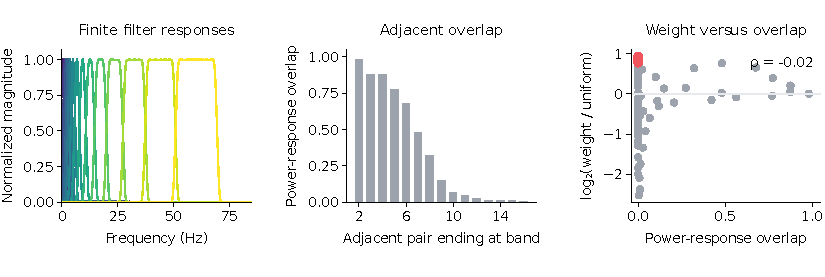
\includegraphics[width=\textwidth]{figures/filter_overlap.pdf}
\caption{\textbf{Finite filter responses and relation weights.} Left: magnitude responses normalized separately by each filter's peak. Middle: adjacent-band power-response cosine overlap. Right: log weight enrichment versus overlap; coral rings identify the ten most enriched pairs. All panels use the two-axis TUEV checkpoint analyzed in Figure~\ref{fig:tokenizer-diagnostics}.}
\label{fig:filter-overlap}
\end{figure}

\section{Scope of pretraining}
\label{app:quad-pretrain}
CroFreMo and the replacement host encoders are trained with supervision
from scratch; released-pretrained baselines and the frozen TFM codebook
are separate comparisons. The
tokenizer places no constraint on the pretraining objective an encoder
might use, and masked-latent prediction over its tokens is the obvious
next step; we leave it there, since a pretraining claim would need its
own scratch control under the same downstream schedule.

\section{Corpora and preprocessing}
\label{app:corpora-details}
The benchmark draws on the Temple University Hospital EEG resource and
its task-specific corpora \citep{obeid2016temple,shah2018temple,veloso2017big},
CHB-MIT \citep{shoeb2009application},
the IIIC annotation and classification resource
\citep{ge2021deep,jing2023development}, the ADFD diagnostic
cohort \citep{miltiadous2023dataset}, and the Sleep-EDF and
ISRUC sleep resources \citep{kemp2000analysis,khalighi2016isruc}.
PhysioNet provides access to several of these public physiological
resources \citep{goldberger2000physiobank}. These citations identify the
source datasets; the preprocessing and evaluation splits used here are
specified below.

\begin{table}[!htbp]
\centering
\small
\caption{Corpora. Splits are subject-disjoint throughout; ``official''
denotes the corpus's released subject-disjoint split.}
\label{tab:corpora}
\resizebox{\textwidth}{!}{%
\begin{tabular}{llll}
\toprule
Corpus & Task & Primary metric & Split \\
\midrule
TUSZ & seizure detection (10\,s windows) & AUC-PR & official train/dev/eval \\
CHB-MIT & seizure detection (10\,s windows) & AUC-PR & subject-disjoint \\
TUEV & epileptiform events, 6 classes (5\,s) & Cohen's $\kappa$ & official train/eval, subject split of train \\
IIIC & IIIC patterns, 6 classes (10\,s) & Cohen's $\kappa$ & subject-disjoint, deduplicated \\
TUAR & artifacts, 3 classes & Cohen's $\kappa$ & subject-disjoint \\
TUAB & abnormal EEG, 2 classes & balanced acc.\ & official train/eval \\
TUEP & epilepsy diagnosis, 2 classes & AUROC & subject-disjoint \\
ADFD & AD / FTD / control & balanced acc.\ & subject-disjoint \\
Sleep-EDF & sleep stages, 5 classes (30\,s) & Cohen's $\kappa$ & subject-disjoint \\
ISRUC & sleep stages, 5 classes (30\,s) & Cohen's $\kappa$ & subject-disjoint \\
\bottomrule
\end{tabular}}
\end{table}
\paragraph{Preprocessing.}
Our model and frozen-loader baselines use a shared preprocessing convention: 16 bipolar channels of the temporal-central-parietal
montage where the corpus records it, band-pass 0.3--75\,Hz, a 60\,Hz notch
(50\,Hz for European recordings), resampling to 200\,Hz, and division by
100\,$\mu$V. Two corpora keep their established conventions instead:
CHB-MIT is normalized per window and channel by its 95th percentile, and
Sleep-EDF is kept at 100\,Hz with train-set standardization; its learnable
filterbank is initialized over 0.5--49\,Hz to remain below the 50-Hz Nyquist
frequency. Processed datasets are accompanied by experiment manifests; release
materials must document the actual split membership and preprocessing
used for each reported row.
Native-loader foundation-model runs retain their host pipeline's input
conventions. These adapter measurements must be interpreted with their
recorded cohort and preprocessing rather than assumed to share every
processed example with the frozen pipeline.

\FloatBarrier



\section{Encoder with a band-only attention sub-layer}
\label{app:band-mixer}\label{app:new-controls}
Before the two-axis encoder of Section~\ref{sec:encoder} we used a
three-axis block that adds a third attention sub-layer over the bands of
one electrode (1.6M parameters; the tokenizer, grid, width, depth and
recipe are otherwise identical). Table~\ref{tab:band-mixer-bench} lists
its benchmark scores next to the current two-axis model, using the
reporting convention of the main tables. The two architectures differ in attention factorization and parameter
count; this comparison does not isolate a single information pathway.
Within the band-mixer architecture, measured rotation does not uniformly
outperform identity, as the matched controls below show.

Every checkpoint is validation-selected.

\begin{table}[!htbp]
\centering
\caption{Band-mixer (three-axis) encoder against the two-axis main model. Three-seed entries are mean $\pm$ sample SD; single entries are seed 0 unless marked. Primary metric per corpus as in the main tables.}
\label{tab:band-mixer-bench}
\TableStyle
\begin{tabular}{llcc}
\toprule
Corpus & Metric & Band-mixer (\textbf{1.6}M) & Two-axis (1.2M) \\\midrule
TUEV & $\kappa$ & $0.703\pm0.031$ & $\mathbf{0.711}\pm0.014$ \\
IIIC & $\kappa$ & $\mathbf{0.523}\pm0.008$ & $0.469\pm0.013$ \\
TUSZ & AUC-PR & $\mathbf{0.654}\pm0.015$ & $0.650\pm0.045$ \\
CHB-MIT & AUC-PR & $0.687\pm0.058$ & $\mathbf{0.690}\pm0.017$ \\
TUAR & $\kappa$ & $\mathbf{0.724}\pm0.042$ & $0.704\pm0.015$ \\
Sleep-EDF & $\kappa$ & $\mathbf{0.700}\pm0.010$ & $0.684$ \\
TUEP & AUROC & $\mathbf{0.811}\pm0.021$ & $0.761$ (s1) \\
ADFD & Bal. acc. & $0.460\pm0.022$ & $\mathbf{0.476}$ (s1) \\
CAUEEG & Bal. acc. & $\mathbf{0.543}\pm0.025$ & -- \\
\bottomrule
\end{tabular}
\end{table}

\begin{table}[!htbp]
\centering
\caption{Retrained controls on the band-mixer encoder with a shared seed within each block. Bold: best value within each block. TUEV reports $\kappa$, balanced accuracy, and weighted F1; CHB-MIT reports AUC-PR, balanced accuracy, and AUROC.}
\TableStyle
\begin{tabular}{llccc}
\toprule
Dataset / seed & Variant & Primary & Bal. acc. & Third metric \\\midrule
TUEV / 2 & Full & \textbf{0.715} & \textbf{0.609} & \textbf{0.846} \\
 & Envelope only & 0.714 & 0.596 & 0.844 \\
 & Weights only & 0.643 & 0.600 & 0.812 \\
 & Own phase & 0.532 & 0.499 & 0.755 \\\midrule
CHB-MIT / 2 & Full & \textbf{0.710} & 0.587 & 0.921 \\
 & Envelope only & 0.543 & 0.589 & 0.900 \\
 & Weights only & 0.645 & \textbf{0.636} & \textbf{0.926} \\
 & Own phase & 0.468 & 0.500 & 0.860 \\\midrule
TUEV / 0 & Measured & 0.714 & \textbf{0.681} & 0.851 \\
 & Identity & \textbf{0.729} & 0.604 & 0.856 \\
 & Sample shuffle & 0.601 & 0.486 & 0.786 \\
\midrule
CHB-MIT / 0 & Measured & 0.697 & 0.609 & 0.913 \\
 & Identity & 0.671 & 0.616 & \textbf{0.931} \\
\bottomrule
\end{tabular}
\end{table}
Identity sets the modulation to one. Sample shuffle cyclically exchanges
complete moment tensors across the batch before constructing modulation;
this changes the input--relation correspondence and can introduce training
noise. It is not a pure test of physiological coupling. TUEV seed-2 full
and envelope-only checkpoints peak at evaluation index 0, and weights-only
and own-phase at index 1; all four complete 20 epochs. CHB-MIT own phase
peaks at index 1 (the second evaluation), envelope only at 108, and weights
only at 271; the full model peaks at 209 and stops by patience after
five epochs. These validation-selected checkpoints remain in the comparison.

\paragraph{Longer estimation context at fixed token resolution.}
On the same encoder, keeping 0.25-s tokens and extending only the moment
window to 1\,s raises TUEV $\kappa$ from 0.714 to 0.739 and CHB-MIT
AUC-PR from 0.697 to 0.727; at 5\,s the scores are 0.737 and 0.618. Longer
context can improve the primary metrics without coarsening tokens, but
the gain is not monotonic and TUEV balanced accuracy falls from 0.681 to
0.627 at 1\,s. The comparison establishes neither an optimal
physiological time scale nor superiority on every metric.

\begin{table}[!htbp]
\centering
\caption{Moment-window sensitivity on the band-mixer encoder. Bold: best value per dataset. Token patches remain 50 samples (0.25\,s); only the moment-aggregation length changes. Metrics follow the preceding table.}
\TableStyle
\begin{tabular}{llccc}
\toprule
Dataset & Moment window & Primary & Bal. acc. & Third metric \\\midrule
TUEV & 0.25\,s & 0.714 & \textbf{0.681} & 0.851 \\
 & 1\,s & \textbf{0.739} & 0.627 & \textbf{0.860} \\
 & 5\,s & 0.737 & 0.604 & 0.859 \\\midrule
CHB-MIT & 0.25\,s & 0.697 & 0.609 & \textbf{0.913} \\
 & 1\,s & \textbf{0.727} & \textbf{0.618} & 0.907 \\
 & 5\,s & 0.618 & 0.587 & 0.891 \\
\bottomrule
\end{tabular}
\end{table}


\FloatBarrier
\section{Tensor specification and computational procedure}
\label{app:tensor-spec}
This appendix specifies the reference tokenizer independently of the
schematic. All tensors refer to one forward pass; $B$ is batch size,
$C$ the number of recorded channels, $T$ the number of samples, $n_b$ the
number of bands, $P$ the number of token patches and $K=d/2$. Index order
is important because the moment matrix stores source and target in an
order different from the attention grid. We use zero-based band indices
in the following algorithm and one-based labels in frequency plots.

\begin{table}[!htbp]
\centering\TableStyle
\caption{Tensor dimensions in the reference construction. The source index
$i$ supplies phase; the target index $j$ supplies amplitude and content.}
\begin{tabular}{lll}
\toprule
Quantity & Shape & Interpretation \\\midrule
Input & $B\times C\times T$ & Preprocessed EEG \\
Filtered/analytic signal & $B\times C\times n_b\times T$ & Full-window bands \\
Moment & $B\times C\times P\times n_b\times n_b$ & Last axes: $i,j$ \\
Projected phase & $B\times C\times P\times n_b\times K$ & Complex, shared real map \\
Envelope/waveform content & $B\times C\times P\times n_b\times K$ & Two real tensors \\
Aligned direction & $B\times C\times P\times n_b\times K$ & Complex target features \\
Token grid & $B\times C\times n_b\times P\times d$ & Interleaved real/imaginary \\
\bottomrule
\end{tabular}
\end{table}

For moment construction, one need not compute angles explicitly. With
$A_j^c=A_j-\bar A_j$, a matrix contraction over time gives
$Z_{ij}=c_Z\langle p_i A_j^c\rangle$. Complex conjugation and guarded
normalization provide the phase factor directly. Avoiding an explicit
$\operatorname{atan2}$ is useful near the phase discontinuity, but it does
not remove the need to guard a moment of small magnitude.

\begin{quote}\small
\textbf{Reference forward pass.}
\begin{enumerate}[leftmargin=*,itemsep=3pt]
\item Filter the full EEG window and form analytic signals in float32.
Compute $A=|z|$ and $p=z/\max(|z|,10^{-6})$.
\item Form non-overlapping moment windows. Center target envelopes within
each window and contract them with source phases to obtain $Z$.
\item Independently divide filtered signals, envelopes and phases into
50-sample token patches. Apply the shared projections $L_w,L_a,L_p$.
\item For each target $j>0$, keep $i<j$, normalize $|Z_{ij}|$ over eligible
sources, and combine their phase features with conjugate moment phases.
If the column sum is at most $10^{-8}$, use the unaligned uniform fallback.
\item Set the root's direction to its own projected phase. Normalize each
complex feature by $\max(|u|,10^{-6})$.
\item Multiply $a+iw$ by the normalized direction, interleave real and
imaginary components, and reorder into the electrode--band--patch grid.
\item Add spatial and band-index embeddings; apply temporal attention,
joint row attention, and the feed-forward layer in each encoder block.
\end{enumerate}
\end{quote}

When the moment window spans $m$ token patches, its moment tensor is
repeated across those $m$ patches. The phase and content projections still
operate on individual short patches. Consequently the moments can share
longer context while token-specific content and projected phase remain
local. The implemented replication requires the number of token patches
to be divisible by the number of moment windows. This is a compatibility
condition, not interpolation between arbitrary window lengths.

\section{What the reference-change property does and does not imply}
\label{app:reference-details}
The transformation in Proposition~\ref{prop:invariance} changes the phase
reference of each source analytic representation by a constant
$\delta_i$. It keeps target envelopes and waveform content fixed. For
one source--target pair,
\begin{align}
p_i' &= e^{i\delta_i}p_i, &
Z_{ij}' &= e^{i\delta_i}Z_{ij}, &
\tilde p_i' &= e^{i\delta_i}\tilde p_i.
\end{align}
The last equality relies on the phase projection sharing its real matrix
between the two complex coordinates and having no bias. If the real and
imaginary parts used unrelated matrices or offsets, this cancellation
would generally fail. Because $|Z_{ij}'|=|Z_{ij}|$, the source weights
remain unchanged. Moreover,
\begin{equation}
\frac{(Z_{ij}')^*}{\max(|Z_{ij}'|,\epsilon_w)}\tilde p_i'
=\frac{e^{-i\delta_i}Z_{ij}^*}{\max(|Z_{ij}|,\epsilon_w)}
 e^{i\delta_i}\tilde p_i
=\frac{Z_{ij}^*}{\max(|Z_{ij}|,\epsilon_w)}\tilde p_i.
\end{equation}
Thus the property also survives the individual phase-factor magnitude
guard, provided that the column does not switch to the unaligned fallback.
The column's guard decision itself is unchanged under the reference
transformation. A subsequent normalization of the already invariant $u_j$
retains invariance, including its small-magnitude guard.

\paragraph{Excluded cases.}
The first band uses its own phase and is not invariant to changing that
phase reference. A fallback column averages unaligned phases, so it is
also outside the claim. A transformation that varies within a window
cannot in general be taken outside the time average or linear projection.
The result therefore concerns a constant reference change per source,
not arbitrary phase warping, frequency drift, or perturbation of only $Z$
while leaving $p$ fixed.

\paragraph{Representation convention versus signal transformation.}
Multiplying an analytic signal by a constant phase would also change its
real component if that real component were used to reconstruct the
waveform. The proposition instead concerns a consistent change of the
phase variables used by the relation branch, with content held fixed.
It does not imply invariance to a time shift of the raw EEG, to changes
in the bandpass filter, or to sensor mixing. These transformations may
change amplitude, waveform projections, window membership, or all three.
The property makes the relation branch internally consistent; its clinical
relevance must be assessed by prediction experiments.

\paragraph{Why it differs from positional rotation.}
Rotary position embeddings apply position-dependent rotations in
attention \citep{su2024roformer}. CroFreMo computes a direction from
measured signal relations and applies it to content before encoding.
Both can be implemented with two-dimensional rotations, but their
conditioning variables, locations in the model, and transformation
properties differ. A phase-reference property alone is not evidence that
one construction is more predictive than another.

\section{Centering, normalization and finite-window behavior}
\label{app:moment-details}
The centered statistic is a complex covariance-like quantity:
\begin{equation}
Z_{ij}/c_Z=\langle p_i A_j\rangle-\langle p_i\rangle\langle A_j\rangle.
\end{equation}
If the envelope is constant within the window, this expression is exactly
zero regardless of the phase samples. In contrast, an uncentered moment
would retain $\bar A_j\langle p_i\rangle$. This matters in subcycle
windows, where the average phase vector need not vanish. Centering removes
that particular contribution, not every source of apparent dependence.
A varying envelope and a slowly changing phase can still produce a moment
without representing a cycle-averaged physiological coupling process.

The distinction between estimating analytic signals and averaging moments
is essential. The filterbank and FFT operate on the entire EEG window;
only the average defining $Z$ is restricted to the estimation window.
Full-window processing avoids re-estimating the analytic signal separately
on each 50-sample patch. It does not create extra cycles inside that patch.
For a rhythm at frequency $f$, the number of cycles in an estimation
window of duration $L$ seconds is $fL$.

\begin{table}[!htbp]
\centering\TableStyle
\caption{Cycle counts implied by the tested moment durations. These are
arithmetic quantities, not a physiological sufficiency criterion.}
\begin{tabular}{lrrrrr}
\toprule
Window & 0.5 Hz & 1 Hz & 2 Hz & 4 Hz & 8 Hz \\\midrule
0.25 s & 0.125 & 0.25 & 0.5 & 1 & 2 \\
1 s & 0.5 & 1 & 2 & 4 & 8 \\
5 s & 2.5 & 5 & 10 & 20 & 40 \\
\bottomrule
\end{tabular}
\end{table}

\paragraph{Relative strength is not confidence.}
Multiplying all moments in one eligible target column by a positive
constant leaves its normalized relative weights unchanged, provided the
guards remain inactive. The conjugate phases are also unchanged. This
explains why the scale $c_Z$ does not ordinarily control token magnitude.
It also means that two columns with very different absolute moment
strengths can produce the same direction. A confidence-weighted gate would
be a different model; the current method should not be described as one.

\paragraph{Cancellation and gradients.}
Even when every individual source moment is nonzero, the weighted
phase-feature sum can nearly cancel. The final guard prevents division by
zero but allows feature attenuation when $|u|<\epsilon$. Above that guard,
$q\mapsto q u/|u|$ preserves pairwise magnitude for a fixed direction.
The end-to-end derivative also includes the dependence of $u$ on the
input and learned parameters; it is not generally an orthogonal map on
raw EEG. Neither the magnitude identity nor reference invariance implies
invertibility of learned projections or the entire tokenizer.

\paragraph{Measurement boundaries.}
Filter overlap, nonstationarity, harmonics of nonsinusoidal waveforms, and
shared sources can all affect phase--amplitude statistics
\citep{aru2015untangling,cole2017brain}. Our response plots and input
interventions examine specific computational questions. They neither
validate a biomarker nor isolate a physiological interaction.

\section{Control definitions and interpretation}
\label{app:control-definition}
A matched control specifies both the tensor that changes and the tensors
that remain available. Let $q_j=a_j+iw_j$ and let $\mathcal N(u)$ denote
$u/\max(|u|,\epsilon)$. The following definitions apply to the reference
rotation construction, with the root and fallback exceptions described
in the method. They should not be conflated with complete changes of
encoder or training pipeline.

\begin{table}[!htbp]
\centering\TableStyle
\caption{Modulation and content in the examined controls.}
\begin{tabular}{lp{0.65\textwidth}}
\toprule
Variant & Token construction \\\midrule
Measured & $h_j=q_j\mathcal N(\sum_{i<j}\alpha_{ij}\eta_{ij}\tilde p_i)$ \\
Identity & $h_j=q_j$, including the root band \\
Own phase & $h_j=q_j\mathcal N(\tilde p_j)$ \\
Weights only & $h_j=q_j\mathcal N(\sum_{i<j}\alpha_{ij}\tilde p_i)$ \\
Envelope only & $h_j=a_j\mathcal N(\sum_{i<j}\alpha_{ij}\eta_{ij}\tilde p_i)$ \\
Sample shuffle & Measured construction with the complete $Z$ tensor
cyclically reassigned along the sample axis \\
\bottomrule
\end{tabular}
\end{table}

\paragraph{Identity and own phase answer different questions.}
Identity removes modulation while preserving envelope and waveform
features. Own phase supplies a different rotation. A loss from own phase
may therefore reflect the difficulty introduced by unaligned rotations;
it cannot, by itself, establish an advantage over unrotated content.
Measured versus identity is the relevant direct comparison for that
question. Identity retains allocated parameter tensors, but its phase
projection is inactive; equal allocated parameter count is not identical
functional use of every parameter.

\paragraph{Weights only isolates one part of the operator.}
It preserves the measured relative magnitudes while removing the
conjugate alignment factors. It still mixes complex source phases and
then normalizes their sum. It is not the same as concatenating a vector
of PAC magnitudes to ordinary EEG features. Thus a measured advantage
against weights only supports the angle's contribution within this
operator, not superiority over every PAC-as-feature approach.

\paragraph{Envelope only tests retained content.}
The waveform coordinate is set to zero; the envelope, phase projections,
moments and downstream grid remain available. Because the waveform
projection starts at zero in the full model, both variants have the same
initial content in that coordinate. Their trained predictions can still
differ through all parameters updated downstream of the construction.
A small difference does not prove that waveform features are identically
zero or useless under other tasks or schedules.

\paragraph{Retraining versus inference intervention.}
Retrained controls adapt their weights to the altered construction.
Inference interventions keep the trained predictor fixed and alter its
inputs or intermediate tensors only at evaluation. The latter measure
reliance and distribution sensitivity. They do not estimate the best
performance obtainable by retraining the alternative. A cyclic sample
shuffle preserves each batch's collection of moment tensors but breaks
their correspondence with EEG windows; it also introduces a different
training distribution when used throughout training.

\section{Parameter counts and computational scaling}
\label{app:complexity}
The parameter column uses the evaluated TUEV configuration, including its
classifier. It avoids comparing an encoder-only count for one method to a
complete classifier for another. Heads that depend on input length or
channel count can change size across tasks. The numbers therefore describe
one common reporting configuration, not immutable sizes of model families.

\begin{table}[!htbp]
\centering\TableStyle
\caption{Parameter comparison reproduced from the main tables. Ratios use
the displayed 1.22M CroFreMo count and are rounded to one decimal.}
\begin{tabular}{lrr}
\toprule
Model & Trainable parameters (M) & Relative to CroFreMo \\\midrule
CroFreMo & 1.22 & 1.0 \\
TFM-Tokenizer & 1.89 & 1.5 \\
BIOT & 3.19 & 2.6 \\
LaBraM & 5.82 & 4.8 \\
CBraMod & 17.9 & 14.7 \\
EEGPT & 25.7 & 21.1 \\
REVE & 69.5 & 57.0 \\
\bottomrule
\end{tabular}
\end{table}

Small parameter count does not imply the fewest operations. The explicit
band grid contains $R P$ tokens with $R=C n_b$. Ignoring projection terms,
temporal attention has score-matrix size proportional to $R P^2$ and
joint row attention to $P R^2$ per head and example. Unfactorized attention
over all tokens would have size $(R P)^2$. With $C=16$, $n_b=16$ and
$P=20$, these are 102,400 temporal scores, 1,310,720 row scores, and
26,214,400 unfactorized scores. The two factored score matrices together
contain approximately 18.6 times fewer entries. This is an arithmetic
comparison of attention layouts, not a measured speedup over the baselines.

Linear projections and feed-forward layers add work proportional to
$RPd^2$. A direct FIR filterbank uses work proportional to $C n_b T L_f$,
where $L_f=201$; the analytic FFT scales approximately as
$C n_b T\log T$. Direct moment construction includes a term proportional
to $C n_b^2 T$. These expressions explain why adding bands can increase
runtime even when the number of learned filter parameters is small.

Memory depends on implementation, precision, batch size, activation
checkpointing and attention kernels. A dense score matrix need not be
materialized by every attention implementation. We consequently do not
convert these counts into claimed GPU memory or throughput results.
Such a benchmark would require the same hardware, input dimensions,
batch size, precision and timing protocol for every model, with warmup
excluded and preprocessing boundaries stated.

\section{Metrics and aggregation}
\label{app:metric-definitions}
Let $M_{ab}$ be the confusion matrix with true class $a$ and predicted
class $b$, and let $N$ be its total count. Balanced accuracy is the mean
class recall, $K^{-1}\sum_a M_{aa}/\sum_b M_{ab}$. Weighted F1 is the
support-weighted average of per-class F1. Cohen's $\kappa$ adjusts observed
agreement $p_o$ by agreement expected from the two marginal distributions,
$p_e$:
\begin{equation}
\kappa=\frac{p_o-p_e}{1-p_e},\qquad
p_o=\frac{\sum_aM_{aa}}{N},\quad
p_e=\frac{\sum_a(\sum_bM_{ab})(\sum_bM_{ba})}{N^2}.
\end{equation}
These metrics emphasize different aspects of class imbalance. High weighted
F1 or $\kappa$ does not establish uniformly high recall for every class.
Conversely, changing decision thresholds can alter balanced accuracy
without changing the ranking of scores used by AUROC.

For seizure detection the primary quantity is trapezoidal area under the
precision--recall curve, computed from continuous class scores. This is
not interchangeable with average precision, which uses a step-weighted
sum of precision values. The main tables retain their recorded AUC-PR
convention throughout. Numbers computed by different integration rules
should not be silently pooled into the same comparison. AUROC and
balanced accuracy are reported alongside it to show complementary behavior.
For TUEP, AUROC is the recorded primary metric; all three binary metrics
remain visible so that a favorable ranking metric does not conceal a
weak decision rule.

\paragraph{Across-run summaries.}
For scores $x_1,\ldots,x_n$, the mean is $\bar x=n^{-1}\sum_sx_s$ and the
sample SD is $s_x=\sqrt{\sum_s(x_s-\bar x)^2/(n-1)}$. A value without a
spread is a single run, not a zero-variance estimate. We report multiple
metrics from the same run or run set; selecting a different run for each
metric would not describe an executable model. Bold identifies the largest
displayed mean or score within the stated comparison, with displayed ties
included. It is not a test of superiority.

\paragraph{Paired comparisons.}
For matched seed indices, define $d_s=x_s-y_s$ before computing
$\bar d$ and $s_d$. In general,
$s_d^2=s_x^2+s_y^2-2\operatorname{Cov}(x,y)$, so the SD of a paired
difference cannot be recovered from the two marginal SDs alone. We use
recorded per-seed pairs where available; a difference between aggregate
means is labeled as such. Three pairs describe observed variability but
provide limited precision, and a confidence interval containing zero is
not evidence of equivalence.

\paragraph{Evaluation unit.}
The displayed window-level metrics weight windows, not subjects, equally.
Correlated windows from one recording do not constitute independent
subjects. Subject-level bootstrap intervals would require membership
records and a specified resampling unit; they are not inferred from the
reported seed SDs. The results do not establish prospective clinical
performance or independence from dataset-specific prevalence.

\section{Comparison scope and training endpoints}
\label{app:comparison-scope}
The paper contains several kinds of comparison, and they support different
claims. A common dataset name is not sufficient to establish that every
row uses identical processed windows. The shared-pipeline supervised
comparison, released-model adaptation, and native-host replacement should
be distinguished when interpreting numerical ranks.

\begin{table}[!htbp]
\centering\TableStyle
\caption{Interpretation of the comparison families.}
\begin{tabular}{lp{0.64\textwidth}}
\toprule
Comparison & Question addressed \\\midrule
Shared-pipeline supervised models & How the reference architecture compares
under the recorded preprocessing and supervised recipes. \\
Released-pretrained models & How the released systems perform under their
recorded adaptation pipelines; preprocessing and pretraining differ. \\
Measured versus identity frontend & Whether modulation helps within a
specified replacement frontend, host and training recipe. \\
Native versus replacement frontend & Whether the complete new frontend
helps the host; this includes band decomposition and adapter effects. \\
Test-time intervention & How a fixed predictor reacts when one part of
its learned input construction changes. \\
\bottomrule
\end{tabular}
\end{table}

\paragraph{Recipes and tuning.}
CroFreMo uses the stated augmentation and regularization settings;
baselines use recorded model-specific recipes. This is not an equal
hyperparameter-search-budget study. A native frontend and a replacement
can also prefer different learning rates or regularization. Such tuning
may change their relative performance. Our comparisons report the
examined settings rather than an upper bound on any baseline's capability.

\paragraph{Validation peaks.}
A checkpoint selected at the first evaluation is a valid outcome of the
stated validation rule, but an informative optimization symptom. It does
not automatically invalidate a result, and it does not demonstrate that
longer training is beneficial. Likewise, a later validation peak does not
prove the absence of other training problems. The TUEV host comparisons
retain first-evaluation peaks rather than selectively rerunning the seed
with the least favorable test score.

\paragraph{Stopping conditions.}
Patience, a fixed epoch limit and a wall-clock budget define different
endpoints. Validation selection within each run is compatible with all
three, but it does not make unequal endpoints an equal-budget comparison.
CHB-MIT controls with different stopping conditions are interpreted
accordingly. A run stopped by a compute budget may provide a useful
predictor while leaving its asymptotic performance unknown.

\paragraph{Checkpoint selection and development.}
Within-run checkpoint selection uses validation. Dataset-level development
also included exploratory architectures and recipes; the benchmark is not
presented as a preregistered evaluation on a never-inspected test suite.
External comparisons therefore remain conditional on the recorded protocol.
A release needs configuration and split manifests alongside weights,
not only the strongest checkpoint.

\section{Paired host results and task dependence}
\label{app:host-pairs}
The following seed-resolved results retain the recorded measured--identity
comparisons in BIOT, including CHB-MIT, where modulation reduces AUC-PR.
They complement the rounded aggregate frontends in
Figure~\ref{fig:host-reuse}. TUEV and IIIC use $\kappa$; CHB-MIT uses AUC-PR.

\begin{table}[!htbp]
\centering\TableStyle
\caption{Recorded BIOT measured--identity seed pairs. Deltas are computed
before rounding; summary SD is across paired differences.}
\begin{tabular}{llrrr}
\toprule
Corpus & Seed & Measured & Identity & Difference \\\midrule
TUEV & 0 & 0.596107 & 0.399942 & +0.196165 \\
 & 1 & 0.582874 & 0.385040 & +0.197834 \\
 & 2 & 0.652658 & 0.442964 & +0.209694 \\
 & Mean $\pm$ SD & $0.611\pm0.037$ & $0.409\pm0.030$ & $+0.201\pm0.007$ \\\midrule
IIIC & 0 & 0.399553 & 0.278632 & +0.120921 \\
 & 1 & 0.366539 & 0.280583 & +0.085956 \\
 & 2 & 0.389959 & 0.244281 & +0.145678 \\
 & Mean $\pm$ SD & $0.385\pm0.017$ & $0.268\pm0.020$ & $+0.118\pm0.030$ \\\midrule
CHB-MIT & 0 & 0.473792 & 0.685205 & $-0.211413$ \\
 & 1 & 0.453602 & 0.646232 & $-0.192630$ \\
 & 2 & 0.465113 & 0.554469 & $-0.089356$ \\
 & Mean $\pm$ SD & $0.464\pm0.010$ & $0.629\pm0.067$ & $-0.164\pm0.066$ \\
\bottomrule
\end{tabular}
\end{table}

Measured exceeds identity in all three recorded TUEV and IIIC pairs and
trails it in all three CHB-MIT pairs. The smaller measured-arm spread on
CHB-MIT does not remove the negative mean difference: it describes
consistent performance at a lower level in these runs. A general claim
that the frontend improves every host or task would therefore be too
strong. The result supports architectural compatibility and task-dependent
predictive utility.

All three TUEV BIOT measured runs select their first validation evaluation.
The identity runs peak at indices 2, 12 and 0; their total epoch counts
are 8, 18 and 6, while the measured runs finish after 6 epochs under the
host's patience rule. First-evaluation selection is therefore disclosed
for both arms. Longer training is not necessarily an advantage when the
validation curve declines. These endpoints do not isolate the reason
for the measured--identity gap.

For native CBraMod versus the CroFreMo replacement, the recorded paired
$\kappa$ differences are $+0.023\pm0.020$ on TUEV and
$-0.012\pm0.007$ on IIIC. Two TUEV replacement runs select the first
validation checkpoint; the three IIIC replacement runs peak later.
These are complete-frontend comparisons. Without a matched CBraMod
identity result in the figure, they cannot attribute a change specifically
to rotation. We do not substitute BIOT attribution for the missing
host-specific comparison.


\section{Full values underlying the summary figures}
\label{app:display-values}
The following tables retain the numerical values shown in the main-text
bar plots. They allow exact lookup without estimating bar heights. Each
metric uses the same reported run aggregation as its source figure; these
tables do not introduce additional evaluations. Differences between two
reported means are descriptive unless seed-level pairing is explicitly
provided.

\begin{table}[!htbp]
\centering\TableStyle
\caption{TUEV component values from Figure~\ref{fig:main-alignment}. Bold marks the highest mean per metric.}
\begin{tabular}{lccc}\toprule
Variant & Balanced Accuracy & $\kappa$ & Weighted F1 \\ \midrule
Measured & $\mathbf{0.650}\pm0.035$ & $\mathbf{0.711}\pm0.014$ & $\mathbf{0.851}\pm0.008$ \\
Own phase & $0.531\pm0.025$ & $0.601\pm0.022$ & $0.789\pm0.016$ \\
Weights only & $0.573\pm0.023$ & $0.662\pm0.020$ & $0.813\pm0.014$ \\
Envelope only & $0.627\pm0.022$ & $0.704\pm0.019$ & $0.843\pm0.013$ \\
Identity & $0.564\pm0.024$ & $0.612\pm0.021$ & $0.768\pm0.017$ \\
\bottomrule\end{tabular}\end{table}

\begin{table}[!htbp]
\centering\TableStyle
\caption{CHB-MIT component values from Figure~\ref{fig:main-alignment}. Bold marks the highest mean per metric.}
\begin{tabular}{lccc}\toprule
Variant & Balanced Accuracy & AUC-PR & AUROC \\ \midrule
Measured & $\mathbf{0.664}\pm0.023$ & $0.690\pm0.017$ & $\mathbf{0.931}\pm0.008$ \\
Own phase & $0.645\pm0.020$ & $0.507\pm0.026$ & $0.882\pm0.011$ \\
Weights only & $0.657\pm0.021$ & $\mathbf{0.692}\pm0.017$ & $0.926\pm0.009$ \\
Envelope only & $0.591\pm0.024$ & $0.562\pm0.024$ & $0.907\pm0.010$ \\
Identity & $0.598\pm0.023$ & $0.650\pm0.019$ & $0.929\pm0.008$ \\
\bottomrule\end{tabular}\end{table}

For TUEV, measured is highest on all three displayed metrics, although the
envelope-only difference is small. On CHB-MIT, measured and weights-only
trade small differences in AUC-PR and AUROC, while envelope-only has a
larger primary-metric deficit. Neither observation alone establishes a
physiological separation of task mechanisms. In particular, the CHB-MIT
stopping-condition caveat applies to this numerical presentation as it
does to the figure.

\FloatBarrier

\begin{table}[!htbp]
\centering\TableStyle
\caption{TUEV frontend-replacement values from Figure~\ref{fig:host-reuse}. Bold marks the highest mean within each host.}
\begin{tabular}{llccc}\toprule
Host & Frontend & Balanced accuracy & $\kappa$ & Weighted F1 \\ \midrule
BIOT & Native & $\mathbf{0.535}\pm0.062$ & $0.532\pm0.025$ & $0.761\pm0.013$ \\
 & Identity & $0.414\pm0.020$ & $0.409\pm0.030$ & $0.696\pm0.015$ \\
 & TFM-Tokenizer & $0.429\pm0.013$ & $0.449\pm0.020$ & $0.708\pm0.012$ \\
 & CroFreMo & $0.530\pm0.019$ & $\mathbf{0.611}\pm0.037$ & $\mathbf{0.796}\pm0.022$ \\
\midrule
CBraMod & Native & $\mathbf{0.574}\pm0.010$ & $0.564\pm0.024$ & $0.767\pm0.004$ \\
 & CroFreMo & $0.539\pm0.018$ & $\mathbf{0.587}\pm0.043$ & $\mathbf{0.784}\pm0.020$ \\
\bottomrule\end{tabular}\end{table}

\begin{table}[!htbp]
\centering\TableStyle
\caption{IIIC frontend-replacement values from Figure~\ref{fig:host-reuse}. Bold marks the highest mean within each host.}
\begin{tabular}{llccc}\toprule
Host & Frontend & Balanced accuracy & $\kappa$ & Weighted F1 \\ \midrule
BIOT & Native & $0.460\pm0.014$ & $0.356\pm0.014$ & $0.462\pm0.015$ \\
 & Identity & $0.384\pm0.018$ & $0.268\pm0.020$ & $0.389\pm0.018$ \\
 & TFM-Tokenizer & $0.460\pm0.009$ & $0.354\pm0.012$ & $0.456\pm0.008$ \\
 & CroFreMo & $\mathbf{0.489}\pm0.017$ & $\mathbf{0.385}\pm0.017$ & $\mathbf{0.488}\pm0.015$ \\
\midrule
CBraMod & Native & $\mathbf{0.489}\pm0.005$ & $\mathbf{0.393}\pm0.006$ & $\mathbf{0.497}\pm0.004$ \\
 & CroFreMo & $0.478\pm0.005$ & $0.382\pm0.004$ & $0.484\pm0.005$ \\
\bottomrule\end{tabular}\end{table}

\begin{table}[!htbp]
\centering\TableStyle
\caption{TUSZ frontend-replacement values from Figure~\ref{fig:host-reuse}. Bold marks the highest mean within each host.}
\begin{tabular}{llccc}\toprule
Host & Frontend & Balanced accuracy & AUC-PR & AUROC \\ \midrule
BIOT & Native & $\mathbf{0.616}\pm0.065$ & $0.347\pm0.026$ & $0.826\pm0.017$ \\
 & Identity & $0.550\pm0.015$ & $0.391\pm0.019$ & $0.829\pm0.015$ \\
 & TFM-Tokenizer & -- & -- & -- \\
 & CroFreMo & $0.517\pm0.023$ & $\mathbf{0.396}\pm0.014$ & $\mathbf{0.845}\pm0.038$ \\
\midrule
CBraMod & Native & $0.576\pm0.049$ & $0.482\pm0.052$ & $0.875\pm0.033$ \\
 & CroFreMo & $\mathbf{0.580}\pm0.030$ & $\mathbf{0.552}\pm0.013$ & $\mathbf{0.904}\pm0.020$ \\
\bottomrule\end{tabular}\end{table}

TFM-Tokenizer on IIIC has two recorded seeds; its TUEV entry has three.
The TUSZ TFM replacement has no reported result in this version. A missing
bar or dash is not a zero score. The replacement figures use each host's
recorded recipe, so differences between BIOT and CBraMod panels should
not be interpreted as a controlled comparison of the hosts themselves.

The BIOT measured--identity summaries in TUEV and IIIC are complemented by
the seed-level pairs in Appendix~\ref{app:host-pairs}. The displayed TUSZ
means do not provide a paired uncertainty estimate by themselves. The
native CBraMod comparisons additionally change the frontend structure,
so they are evidence about whole-frontend reuse rather than a direct
measured--identity attribution within that host.


\FloatBarrier
\section{Fixed-checkpoint diagnostic protocol and complete outputs}
\label{app:diagnostic-protocol}
The diagnostic checkpoint is the validation-selected seed-0 instance of
the two-axis reference architecture with 16 bands and 50-sample token and
moment windows. Its test $\kappa$ is 0.684601, distinct from the
0.711 mean of the current main-table aggregation. No diagnostic intervention
changes which checkpoint is selected, and none is included as another
seed in a benchmark mean. The analysis first strictly reloads the state
dictionary, then checks that an identity analysis hook leaves logits
unchanged. The unchanged full-test evaluation reproduces each archived
checkpoint metric to within $10^{-6}$.

All 29,421 processed test windows are used. A fixed, label-independent
permutation (random seed 20260916) orders windows into batches of 32.
Shuffling cyclically moves each whole moment tensor by one sample within
its batch; electrodes, patches and band-pair axes inside the tensor stay
together. The final batch is retained and has more than one sample.
This is a cross-window diagnostic, not a cross-subject surrogate analysis.
All other interventions share exactly the same window ordering.

\begin{table}[!htbp]
\centering\TableStyle
\caption{Fixed-checkpoint interventions on TUEV. These are inference
changes to one trained predictor, not independently trained models.}
\begin{tabular}{lccc}\toprule
Intervention & Balanced accuracy & $\kappa$ & Weighted F1 \\\midrule
Unchanged & \textbf{0.636580} & \textbf{0.684601} & \textbf{0.835755} \\
Identity & 0.166667 & 0.000000 & 0.534726 \\
Own phase & 0.239098 & 0.215510 & 0.620810 \\
Weights only & 0.445144 & 0.416021 & 0.689325 \\
Shuffled moments & 0.252590 & 0.174059 & 0.589881 \\
Envelope only & 0.425864 & 0.623135 & 0.791911 \\
\bottomrule\end{tabular}\end{table}

The identity intervention predicts the background class for every window,
which yields balanced accuracy $1/6$ and $\kappa=0$. This is a distribution
shift in a predictor trained with modulation. The retrained identity
models in Figure~\ref{fig:main-alignment} are different predictors and do
not have that degenerate result. Confusing these two experiments would
turn a reliance diagnostic into an unsupported training claim.

\paragraph{Averaging the relation weights.}
Weights are first averaged over electrodes and patches within each window,
then equally over windows. Each non-root target has source weights summing
to one. For target index $j>0$, uniform source weighting assigns $1/j$ to
each of its $j$ eligible sources. The heat map plots
$\log_2(\bar\alpha_{ij}/(1/j))$, which prevents targets with different
numbers of sources from being compared by raw weight alone. The
frequency-ratio histogram gives each of the 15 non-root targets equal
total mass. Its bins use nominal cutoff midpoints, not peak frequencies.

\paragraph{Edge sensitivity and numerical fallback.}
Removing the first and last two token patches from the weight summary
changes any mean coefficient by at most 0.001894. This is a sensitivity
check on the summary, not proof of accurate edge phase. The fraction of
eligible target columns using the small-moment fallback is approximately
$7.1\times10^{-9}$ in this evaluation. An infrequent numerical fallback
does not mean that all above-threshold moments are physiologically strong.

\FloatBarrier
\subsection{Class-wise behavior and waveform content}
The test set is imbalanced: background accounts for 19,646 of 29,421
windows. Class-resolved results therefore add information beyond weighted
F1. The unchanged checkpoint has low SPSW F1 despite its stronger aggregate
metrics. It would be inappropriate to infer uniform improvement across
all epileptiform categories from the aggregate $\kappa$ alone.

\begin{table}[!htbp]
\centering\TableStyle
\caption{Per-class F1 under fixed-checkpoint inference interventions.}
\begin{tabular}{lrrrrrr}\toprule
Intervention & SPSW & GPED & PLED & EYEM & ARTF & BCKG \\\midrule
Unchanged & \textbf{0.057} & \textbf{0.817} & \textbf{0.585} & \textbf{0.773} & \textbf{0.545} & \textbf{0.922} \\
Identity & 0.000 & 0.000 & 0.000 & 0.000 & 0.000 & 0.801 \\
Own phase & 0.000 & 0.389 & 0.023 & 0.158 & 0.010 & 0.831 \\
Weights only & 0.000 & 0.480 & 0.195 & 0.258 & 0.516 & 0.836 \\
Shuffled moments & 0.000 & 0.040 & 0.011 & 0.046 & 0.517 & 0.814 \\
Envelope only & 0.006 & 0.791 & 0.421 & 0.100 & 0.384 & 0.910 \\
Test windows & 567 & 4677 & 1998 & 329 & 2204 & 19646 \\
\bottomrule\end{tabular}\end{table}

\begin{figure}[!htbp]
\centering
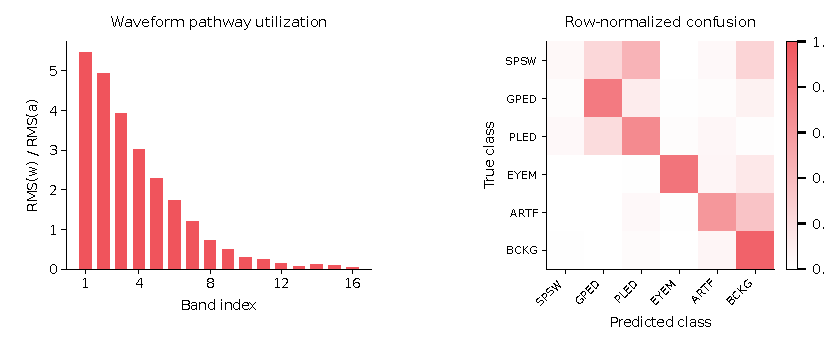
\includegraphics[width=\textwidth]{figures/content_and_confusion.pdf}
\caption{\textbf{Content use and class errors in the diagnostic checkpoint.}
Left: ratio of waveform to envelope feature RMS, aggregated over the full
test set. Right: row-normalized confusion matrix of unchanged predictions.
These are measurements of one fixed checkpoint, not the aggregate main-table model.}
\end{figure}

A nonzero waveform RMS shows that the zero-initialized projection became
active. It does not establish that the waveform contribution is uniquely
necessary: correlated information may be present in the envelope, phase
and other bands. The retrained envelope-only comparison and the inference
intervention address adaptation and immediate reliance, respectively, and
need not have the same effect size. RMS ratios are feature-scale
measurements, not fractions of explained predictive performance.

\subsection{Filter-by-filter responses}
Figure~\ref{fig:all-responses} compares initialized and trained finite
responses in each band. The horizontal scale is local to the band so that
the low-frequency response shapes remain visible. Each curve is normalized
to its own peak; shading marks the trained nominal cutoff interval. Thus
neither the curve height nor the shaded interval should be read as a
learned coupling strength or an uncertainty interval.

\begin{figure}[!htbp]
\centering
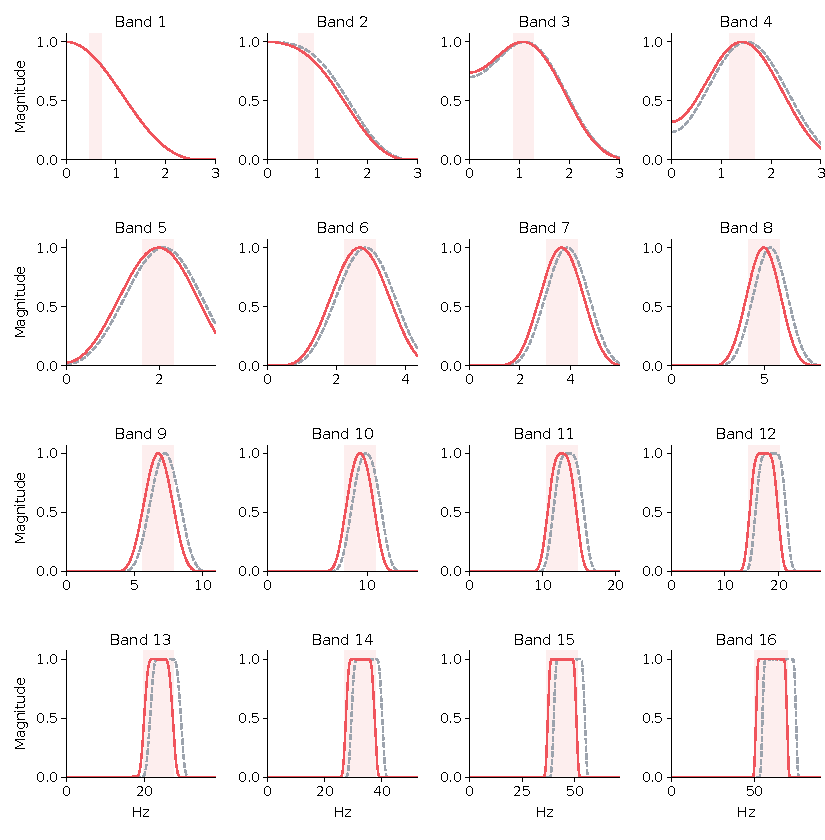
\includegraphics[width=\textwidth]{figures/all_filter_responses.pdf}
\caption{\textbf{Actual finite responses for all sixteen filters.} Dashed gray:
initialization. Coral: trained response. Shading: trained nominal cutoff
interval. Curves are individually normalized and frequency axes differ
between panels. This separates cutoff ordering from spectral separation.}
\label{fig:all-responses}
\end{figure}

\FloatBarrier

\section{Audited reference configuration}
\label{app:reference-config}
The following configuration and parameter decomposition were read from
the diagnostic checkpoint and its corresponding model implementation.
They specify the reference TUEV architecture and training settings; they
do not imply that every host or every corpus uses identical stopping,
loss or input conventions.

\begin{table}[!htbp]
\centering\TableStyle
\caption{Reference TUEV settings.}
\begin{tabular}{ll}\toprule
Component & Setting \\\midrule
Sampling / input & 200 Hz; 16 channels; 5-s windows \\
Filterbank & 16 filters; length 201; initial range 0.5--75 Hz \\
Token / moment window & 50 / 50 samples \\
Content width & 64 envelope + 64 waveform features \\
Encoder & 6 blocks; 4 heads; temporal and joint row attention \\
Feed-forward width & 256, with GELU \\
Band embedding & Learned band-index embedding \\
Spatial embedding & Coordinate-based embedding \\
Dropout & 0.35 \\
Optimizer & AdamW; learning rate $10^{-4}$; weight decay 0.05 \\
Schedule / gradient clipping & Cosine decay / norm 1.0 \\
Batch / loss & 32 / cross-entropy with label smoothing 0.1 \\
Epoch cap / patience & 20 / 20; validation each epoch \\
\bottomrule\end{tabular}\end{table}

\begin{table}[!htbp]
\centering\TableStyle
\caption{Allocated parameters in the reference diagnostic checkpoint.}
\begin{tabular}{lr}\toprule
Component & Parameters \\\midrule
Tokenizer & 9,760 \\
Band embeddings & 2,048 \\
Spatial embeddings & 17,408 \\
Encoder & 1,194,240 \\
Classifier & 1,030 \\
Total & 1,224,486 \\
\bottomrule\end{tabular}\end{table}

One of five configured augmentations is selected per training forward
pass: time reversal with probability 0.5, Gaussian jitter with scale
0.05, masking 20\% of sample positions, masking 20\% of channels, or
randomly masking approximately 20\% of real-FFT coefficients. The
implementation samples a transform for the forward pass rather than
applying all five sequentially. Evaluation disables these augmentations.
The reference loss, batch size, and epoch settings above are therefore
part of the evaluated recipe, not claims of uniquely optimal values.

\paragraph{Finite-window filtering.}
Convolution uses 100-sample zero padding on each side to preserve signal
length. The Hilbert transform uses a full-window FFT multiplier: DC and,
for even lengths, Nyquist receive weight one; positive frequencies receive
two; negative frequencies receive zero. No additional reflected padding
is inserted around that FFT. The preprocessing bandpass and learned
filterbank are distinct operations. Edge sensitivity remains relevant
because neither zero padding nor the finite-window FFT supplies observed
signal outside the recording window.

\paragraph{Release records.}
A reproducible model record consists of the architecture configuration,
seed, validation selection rule, checkpoint, test metrics, preprocessing
manifest and split membership. A weight file alone does not identify the
window construction or normalization. The diagnostic audit additionally
stores checkpoint, result, manifest and analysis-script hashes locally.
The publication figures omit user names and machine-specific paths;
these are not required to understand the methods or numerical results.


\clearpage
\section{Numerical filter and content summary}
\label{app:filter-numbers}
This table gives the numerical quantities underlying the diagnostic
filter plots. All rows come from the same validation-selected two-axis
TUEV checkpoint; none represents a separate fit or seed. Nominal edges
are trainable cutoff parameters, while response peaks and threshold
spans are measured from the reconstructed finite FIR response. The two
should not be substituted for each other when interpreting a frequency
pair as slow-to-fast.

\begin{table}[!htbp]
\centering\TableStyle
\caption{Trained filter parameters, finite-response measurements and
waveform utilization. Frequencies are in Hz. ``Half-power span'' gives
the outermost frequencies at or above half the peak power. RMS ratios
are computed from the full test-set feature tensors.}
\begin{tabular}{rrrrrrr}
\toprule
Band & \multicolumn{2}{c}{Nominal cutoff} & Response peak & \multicolumn{2}{c}{Half-power span} & RMS ratio \\
 & Low & High & & Low & High & $w/a$ \\\midrule
1 & 0.492 & 0.688 & 0.000 & 0.000 & 0.873 & 5.466 \\
2 & 0.646 & 0.887 & 0.000 & 0.000 & 1.190 & 4.929 \\
3 & 0.904 & 1.258 & 1.068 & 0.000 & 1.740 & 3.912 \\
4 & 1.194 & 1.641 & 1.416 & 0.769 & 2.063 & 3.027 \\
5 & 1.651 & 2.278 & 1.978 & 1.306 & 2.637 & 2.289 \\
6 & 2.250 & 3.096 & 2.667 & 1.990 & 3.351 & 1.729 \\
7 & 3.078 & 4.241 & 3.656 & 2.954 & 4.358 & 1.190 \\
8 & 4.163 & 5.720 & 4.944 & 4.199 & 5.688 & 0.733 \\
9 & 5.699 & 7.817 & 6.757 & 5.914 & 7.605 & 0.483 \\
10 & 7.825 & 10.751 & 9.290 & 8.185 & 10.388 & 0.303 \\
11 & 10.689 & 14.644 & 12.671 & 11.096 & 14.233 & 0.241 \\
12 & 14.568 & 19.920 & 16.785 & 14.972 & 19.513 & 0.144 \\
13 & 19.951 & 27.259 & 22.058 & 20.355 & 26.855 & 0.077 \\
14 & 27.370 & 37.420 & 32.397 & 27.777 & 37.012 & 0.107 \\
15 & 37.232 & 50.871 & 44.049 & 37.640 & 50.464 & 0.085 \\
16 & 50.879 & 69.543 & 52.875 & 51.288 & 69.135 & 0.041 \\
\bottomrule\end{tabular}\end{table}

\paragraph{Response measurement.}
For a finite kernel $h_b[n]$, the plotted response is
$H_b(f)=\sum_n h_b[n]e^{-i2\pi fn/f_s}$. Each magnitude curve is normalized
by its own maximum for display. The half-power set is
$\{f:|H_b(f)|^2\ge\max_{f'}|H_b(f')|^2/2\}$ on the sampled frequency
grid. The table lists its minimum and maximum. If a response has multiple
lobes, this outer span need not be a single contiguous interval. Frequency
resolution is approximately 0.0061 Hz from the 32,768-point transform;
extra transform bins improve display resolution, not the physical
resolving power of the 201-tap kernel.

\paragraph{Order and separation.}
The nominal midpoints remain strictly increasing in this checkpoint.
The first two response peaks are nevertheless both at zero, and the
third band's half-power span includes zero. These observations are
compatible: ordered parameter intervals do not guarantee disjoint
frequency support. Frequency-ratio summaries use nominal midpoints
consistently, while the overlap analysis uses actual power responses.
Neither diagnostic substitutes for checking additional checkpoints or
other sampling rates.

\paragraph{Content scale.}
For band $b$, the reported ratio is
$\sqrt{\mathbb E[w_b^2]/\mathbb E[a_b^2]}$, with expectation over windows,
electrodes, patches and feature coordinates. It establishes whether the
waveform projection has become active after zero initialization. It is
not a percentage contribution to accuracy, and ratios from differently
calibrated feature spaces should not be treated as directly comparable
physiological amplitudes. Predictive necessity is tested by the retrained
controls, with the inference intervention as a separate reliance check.

\end{document}
